%
%   This program is free software: you can redistribute it and/or modify
%   it under the terms of the GNU General Public License as published by
%   the Free Software Foundation, either version 3 of the License, or
%   (at your option) any later version.
%
%   This program is distributed in the hope that it will be useful,
%   but WITHOUT ANY WARRANTY; without even the implied warranty of
%   MERCHANTABILITY or FITNESS FOR A PARTICULAR PURPOSE.  See the
%   GNU General Public License for more details.
%
%   You should have received a copy of the GNU General Public License
%   along with this program.  If not, see <http://www.gnu.org/licenses/>.
%

% Version: $Revision$

\documentclass[a4paper]{book}

\usepackage{epsfig}
\usepackage{wrapfig}
\usepackage{graphicx}
\usepackage{hyperref}

\input{hyphenation}
\input{extensions}

\title{\epsfig{file=images/coat_of_arms.eps,width=10cm}\vspace{3cm}\\WEKA Manual\\for Version 3-9-0}
\author{Remco R. Bouckaert\\Eibe Frank\\Mark Hall\\Richard Kirkby\\Peter Reutemann\\Alex Seewald\\David Scuse}

\setcounter{secnumdepth}{3}
\setcounter{tocdepth}{3}

\begin{document}

\begin{titlepage}
\maketitle

\thispagestyle{empty}
\center
\begin{table}[b]
\copyright 2002-2016 \\
 \\
University of Waikato, Hamilton, New Zealand \\
Alex Seewald (original Commnd-line primer) \\
David Scuse (original Experimenter tutorial) \\
\\
This manual is licensed under the GNU General Public License version 3. More information about this license can be found at \url{http://www.gnu.org/licenses/gpl-3.0-standalone.html}
\end{table}

\end{titlepage}

\tableofcontents

%%%%%%%%%%%%%%%%%%%%%%%%%%%%%%%%%%%
\part{The Command-line}

\chapter{A command-line primer}
\input{commandline}

%%%%%%%%%%%%%%%%%%%%%%%%%%%%%%%%%%%
\part{The Graphical User Interface}

\chapter{Launching WEKA}
%
%   This program is free software: you can redistribute it and/or modify
%   it under the terms of the GNU General Public License as published by
%   the Free Software Foundation, either version 3 of the License, or
%   (at your option) any later version.
%
%   This program is distributed in the hope that it will be useful,
%   but WITHOUT ANY WARRANTY; without even the implied warranty of
%   MERCHANTABILITY or FITNESS FOR A PARTICULAR PURPOSE.  See the
%   GNU General Public License for more details.
%
%   You should have received a copy of the GNU General Public License
%   along with this program.  If not, see <http://www.gnu.org/licenses/>.
%

% Version: $Revision$

The Weka GUI Chooser (class \texttt{weka.gui.GUIChooser}) provides a
starting point for launching Weka's main GUI applications and
supporting tools. If one prefers a MDI (``multiple document
interface'') appearance, then this is provided by an alternative
launcher called ``Main'' (class \texttt{weka.gui.Main}).

%%The new menu-driven GUI in WEKA (class \texttt{weka.gui.Main}) succeeds the old GUI Chooser (class \texttt{weka.gui.GUIChooser}). Its MDI (``multiple document interface'') appearance makes it easier to keep track of all the open windows. If one prefers an SDI (``single document interface'') driven layout, one can invoke this with option \texttt{-gui sdi} on the commandline.

The GUI Chooser consists of four buttons---one for each of the four
major Weka applications---and four menus. 

\begin{center}
	\includegraphics[angle=270,width=5cm]{images/launching/GUIChooser.eps}
\end{center}

The buttons can be used to start the following applications:

		\begin{itemize}
			\item \textbf{Explorer} An environment for exploring data with
WEKA (the rest of this documentation deals with this application in more detail).
			\item \textbf{Experimenter} An environment for performing experiments and conducting statistical tests
between learning schemes.
			\item \textbf{KnowledgeFlow} This environment supports essentially
the same functions as the Explorer but with a drag-and-drop
interface. One advantage is that it supports incremental learning.
                        \item \textbf{Workbench} An all-in-one application that combines all the others
                        within user-selectable ``perspectives''.
			\item \textbf{SimpleCLI} Provides a simple command-line interface
that allows direct execution of WEKA commands for operating systems
that do not provide their own command line interface.
		\end{itemize}




The menu consists of four sections:

\begin{enumerate}
	\item \textbf{Program} \\
	        \includegraphics[angle=270,width=2cm]{images/launching/guic_program.eps}
		\begin{itemize}
			\item \textbf{LogWindow} Opens a log window that captures all that is printed to \textit{stdout} or \textit{stderr}. Useful for environments like MS Windows, where WEKA is normally not started from a terminal.
			\item \textbf{Exit} Closes WEKA.
		\end{itemize}
				
	\item \textbf{Tools} Other useful applications. \\
                \includegraphics[angle=270,width=2cm]{images/launching/guic_tools.eps}
		\begin{itemize}
                        \item \textbf{Package manager} A graphical interface to Weka's package management system.
			\item \textbf{ArffViewer} An MDI application for viewing ARFF files in spreadsheet format.
			\item \textbf{SqlViewer} Represents an SQL worksheet, for querying databases via JDBC.
                        \item \textbf{Bayes net editor} An application for editing, visualizing and learning Bayes nets.
		\end{itemize}
		
	\item \textbf{Visualization} Ways of visualizing data with WEKA. \\
		\includegraphics[angle=270,width=2cm]{images/launching/guic_visualization.eps}
		\begin{itemize}
			\item \textbf{Plot} For plotting a 2D plot of a dataset.
			\item \textbf{ROC} Displays a previously saved ROC curve.
			\item \textbf{TreeVisualizer} For displaying directed graphs, e.g., a decision tree.
			\item \textbf{GraphVisualizer} Visualizes XML BIF or DOT format graphs, e.g., for Bayesian networks.
			\item \textbf{BoundaryVisualizer} Allows the visualization of classifier decision boundaries in two dimensions.
		\end{itemize}
		
		
	\item \textbf{Help} Online resources for WEKA can be found here. \\
	        \includegraphics[angle=270,width=2cm]{images/launching/guic_help.eps}
		\begin{itemize}
			\item \textbf{Weka homepage} Opens a browser window with WEKA's homepage.
			\item \textbf{HOWTOs, code snippets, etc.} The general WekaWiki \cite{wekawiki}, containing lots of examples and HOWTOs around the development and use of WEKA.
			\item \textbf{Weka on Sourceforge} WEKA's project homepage on Sourceforge.net.
			\item \textbf{SystemInfo} Lists some internals about the Java/WEKA environment, e.g., the \texttt{CLASSPATH}.
		\end{itemize}
\end{enumerate}

To make it easy for the user to add new functionality to the menu without having to modify 
the code of WEKA itself, the GUI now offers a plugin mechanism for such add-ons. 
Due to the inherent dynamic
class discovery, plugins only need to implement the \texttt{weka.gui.MainMenuExtension}
interface and WEKA notified of the package they reside in to be displayed in the menu under 
``Extensions'' (this extra menu appears automatically as soon as extensions are discovered). 
More details can be found in the Wiki article ``Extensions for Weka's main GUI'' 
\cite{mainextensions}.

If you launch WEKA from a terminal window, some text begins scrolling in the
terminal. Ignore this text unless something goes wrong, in which case it can
help in tracking down the cause (the \textit{LogWindow} from the \textit{Program} menu 
displays that information as well).

This User Manual focuses on using the Explorer but does not explain
the individual data preprocessing tools and learning algorithms in
WEKA. For more information on the various filters and learning methods
in WEKA, see the book {\em Data Mining} \cite{witten}.


\chapter{Package Manager}
\input{package_manager}

\chapter{Simple CLI}
\input{simplecli}

\chapter{Explorer}
\input{explorer}

\chapter{Experimenter}
\input{experimenter}

\chapter{KnowledgeFlow}
%
%   This program is free software: you can redistribute it and/or modify
%   it under the terms of the GNU General Public License as published by
%   the Free Software Foundation, either version 3 of the License, or
%   (at your option) any later version.
%
%   This program is distributed in the hope that it will be useful,
%   but WITHOUT ANY WARRANTY; without even the implied warranty of
%   MERCHANTABILITY or FITNESS FOR A PARTICULAR PURPOSE.  See the
%   GNU General Public License for more details.
%
%   You should have received a copy of the GNU General Public License
%   along with this program.  If not, see <http://www.gnu.org/licenses/>.
%

% Version: $Revision$

%%%%%%%%%%%%%%%%
% Introduction %
%%%%%%%%%%%%%%%%

\section{Introduction}

The KnowledgeFlow provides an alternative to the Explorer as a
graphical front end to WEKA's core algorithms. Weka 3.8.0 and 3.9.0
contain a new implementation of the KnowledgeFlow - this new
implementation is more efficient, has a simpler API than the old
version, and now lives in the \verb+weka.knowledgeflow+ and
\verb+weka.gui.knowledgeflow+ packages. The old Knowledge Flow
implementation is still available in the \verb+weka.gui.beans+
package.

\begin{center}
  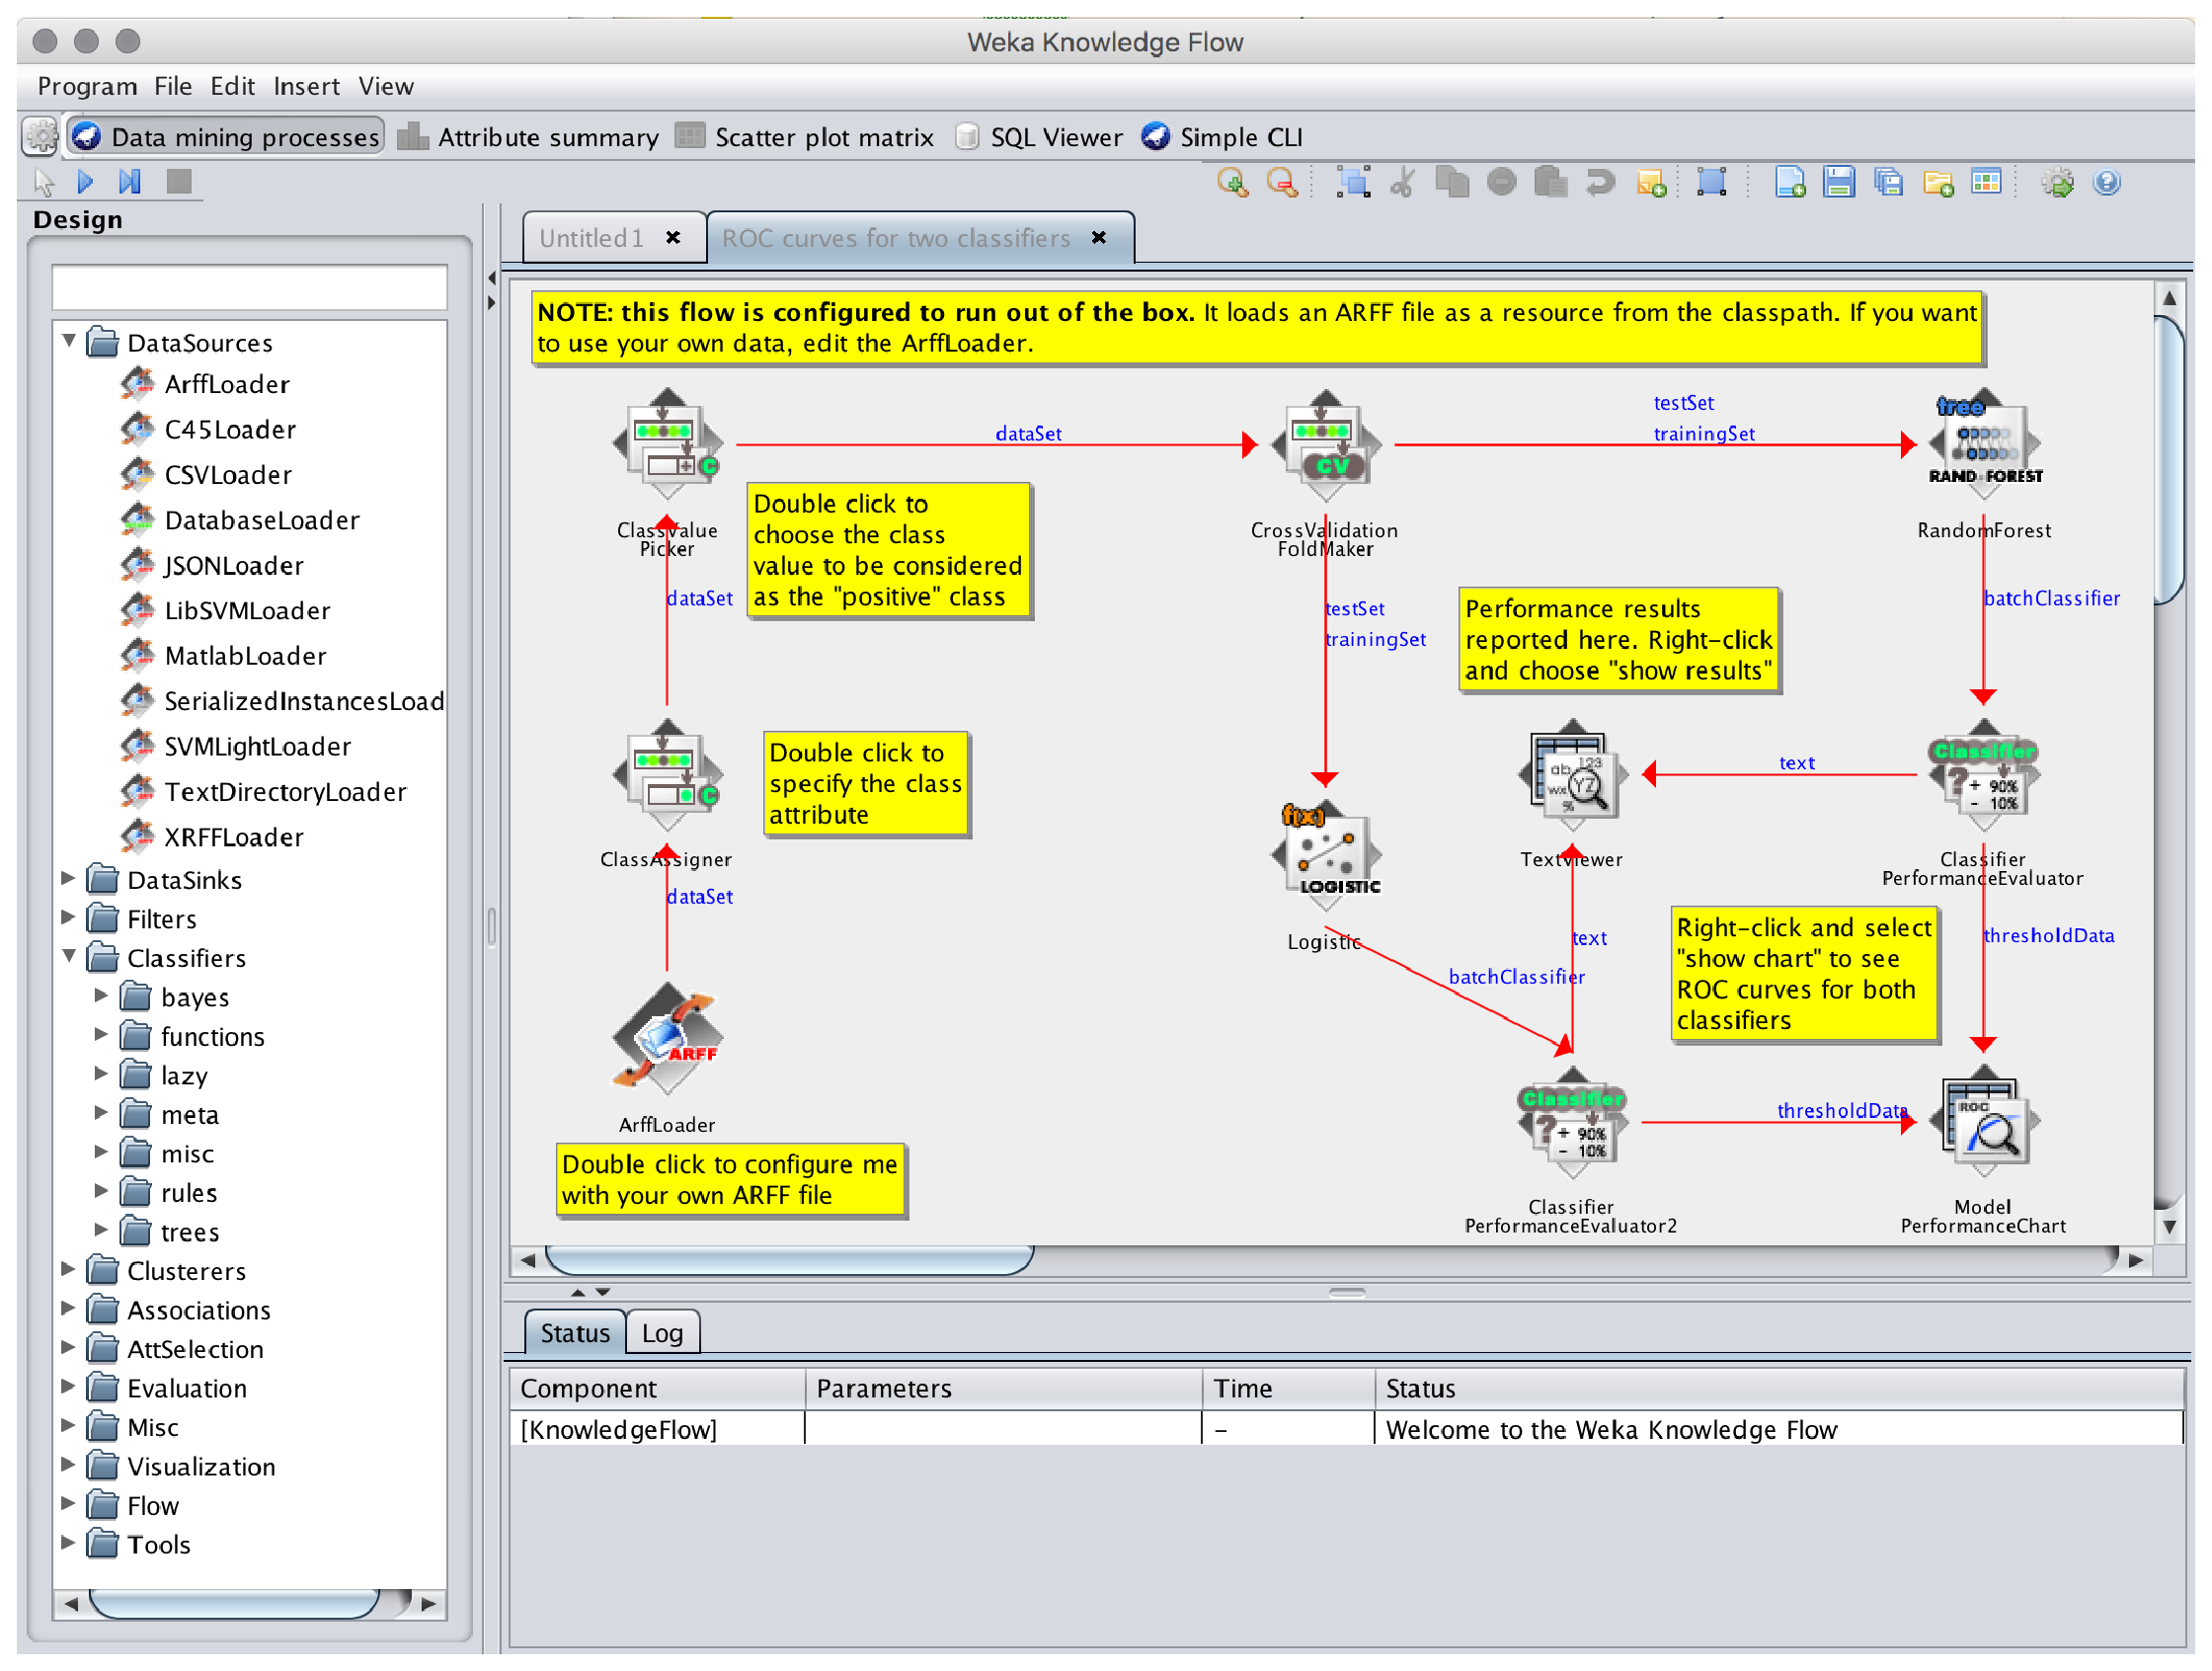
\includegraphics[width=10cm]{images/knowledgeflow/knowledgeflow.eps}
\end{center}

The KnowledgeFlow presents a \textit{data-flow} inspired interface to
WEKA. The user can select WEKA steps from a palette, place them
on a layout canvas and connect them together in order to form a
\textit{knowledge flow} for processing and analyzing data. At present,
all of WEKA's classifiers, filters, clusterers, associators, loaders
and savers are available in the KnowledgeFlow along with some extra
tools.

The KnowledgeFlow can handle data either incrementally or in batches
(the Explorer handles batch data only). Of course learning from data
incrementally requires a classifier that can be updated on an instance
by instance basis. Currently in WEKA there are ten classifiers that
can handle data incrementally:
\begin{tight_itemize}
	\item AODE
	\item IB1
	\item IBk
	\item KStar
	\item NaiveBayesMultinomialUpdateable
	\item NaiveBayesUpdateable
	\item NNge
	\item Winnow
        \item SGD
        \item SPegasos
\end{tight_itemize}

\noindent A further two classifiers are meta classifiers:
\begin{tight_itemize}
	\item \textit{RacedIncrementalLogitBoost} - that can use of any regression base
learner to learn from discrete class data incrementally.
	\item \textit{LWL} - locally weighted learning.
\end{tight_itemize}

Furthermore, other incremental streaming classifiers from the MOA
project are accessible through the ``massiveOnlineAnalysis'' package
(available for installation via the package manager).

%%%%%%%%%%%%
% Features %
%%%%%%%%%%%%

\newpage
\section{Features}

The KnowledgeFlow offers the following features:
\begin{itemize}
	\item intuitive data flow style layout
	\item process data in batches or incrementally 
	\item launch multiple start points in parallel
        \item launch multiple start points sequentially in a user-defined order
        \item fully multi-threaded - each step in a flow executes in its own thread (except for those processing streaming data)
        \item single threaded execution for streaming flows
	\item chain filters together
	\item view models produced by classifiers for each fold in a cross validation
	\item visualize performance of incremental classifiers during 
  	processing (scrolling plots of classification accuracy, RMS error, 
  	predictions etc.)
        \item plugin ``perspectives'' that add major new functionality (e.g. 3D data visualization, 
          time series forecasting environment etc.)
\end{itemize}

\newpage
\section{Flow Steps}
Steps available in the KnowledgeFlow:

\subsection{DataSources} All of WEKA's loaders are available.
%\begin{center}
	%\epsfig{file=images/knowledgeflow/components_datasources.eps,height=2cm}
%\end{center}

\subsection{DataSinks} All of WEKA's savers are available. Along with the
following KnowledgeFlow-specific ones:

\begin{itemize}  
\item \textit{TextSaver} - save text carried by a text connection out to a file.
\item \textit{ImageSaver} - save the image data carried by an image connection
out to a file in either PNG or GIF format.
\item \textit{SerializedModelSaver} - save the classifier or clusterer
  encapsulated in a batchClassifier, incrementalClassifier or batchClusterer
  connection out to a file.
\end{itemize}

\subsection{DataGenerators} All of WEKA's data generators are available.

%\begin{center}
%	\epsfig{file=images/knowledgeflow/components_datasinks.eps,height=2cm}
%\end{center}

\subsection{Filters} All of WEKA's filters are available.
%\begin{center}
%	\epsfig{file=images/knowledgeflow/components_filters.eps,height=2cm}
%\end{center}

\subsection{Classifiers} All of WEKA's classifiers are available.
%\begin{center}
%	\epsfig{file=images/knowledgeflow/components_classifiers.eps,height=2cm}
%\end{center}

\subsection{Clusterers} All of WEKA's clusterers are available.
%\begin{center}
%	\epsfig{file=images/knowledgeflow/components_clusterers.eps,height=2cm}
%\end{center}

\subsection{Attribute selection} All of WEKA's attribute and subset evaluators
are available, along with all of the search methods.

\subsection{Evaluation}
%\begin{center}
%	\epsfig{file=images/knowledgeflow/components_evaluation.eps,height=2cm}
%\end{center}

\begin{itemize}
	\item \textit{TrainingSetMaker} - make a data set into a training set.
	\item \textit{TestSetMaker} - make a data set into a test set.
	\item \textit{CrossValidationFoldMaker} - split any data set, training 
	set or test set into folds.
	\item \textit{TrainTestSplitMaker} - split any data set, training set 
	or test set into a training set and a test set.
        \item \textit{InstanceStreamToBatchMaker} - collects the instances in
          an incoming instance stream and outputs them as a batch set of Instances.
	\item \textit{ClassAssigner} - assign a column to be the class for any 
	data set, training set or test set.
	\item \textit{ClassValuePicker} - choose a class value to be considered 
	as the ``positive'' class. This is useful when generating data for ROC style 
	curves (see \textit{ModelPerformanceChart} below and example \ref{exampleroc}).
	\item \textit{ClassifierPerformanceEvaluator} - evaluate the performance of 
	batch trained/tested classifiers.
	\item \textit{IncrementalClassifierEvaluator} - evaluate the performance of 
	incrementally trained classifiers.
	\item \textit{ClustererPerformanceEvaluator} - evaluate the performance of 
	batch trained/tested clusterers.
	\item \textit{PredictionAppender} - append classifier predictions to a test 
	set. For discrete class problems, can either append predicted class labels or
	probability distributions.
\end{itemize}

\subsection{Visualization}
%\begin{center}
%	\epsfig{file=images/knowledgeflow/components_visualization.eps,height=2cm}
%\end{center}

\begin{itemize}
	\item \textit{DataVisualizer} - a step that can pop up a panel for 
	visualizing data in a single large 2D scatter plot.
	\item \textit{ScatterPlotMatrix} - a step that can pop up a panel 
	containing a matrix of small scatter plots (clicking on a small plot 
	pops up a large scatter plot).
	\item \textit{AttributeSummarizer} - a step that can pop up a panel 
	containing a matrix of histogram plots - one for each of the attributes 
	in the input data.
	\item \textit{ModelPerformanceChart} - a step that can pop up a 
	panel for visualizing threshold (i.e. ROC style) curves.
        \item \textit{CostBenefitAnalysis} - a step that can popup a graphical
          tool for exploring cost/benefit tradeoffs by interactively selecting
          different population sizes from a ranked list of prospects or by 
          varying the threshold on the predicted probability of the positive class. It
          displays both a cumulative gains chart and a cost/benefit plot.
	\item \textit{TextViewer} - a step for showing textual data. Can show 
	data sets, classification performance statistics etc.
	\item \textit{GraphViewer} - a step that can pop up a panel for 
	visualizing tree based models.
	\item \textit{StripChart} - a step that can pop up a panel that displays 
	a scrolling plot of data (used for viewing the online performance of 
	incremental classifiers).
        \item \textit{ImageViewer} - a step that can popup a visualization for static
          image data.
        \item \textit{BoundaryPlotter} - a step that accepts a dataSet, along with one
          or more info connections from classifiers or clusterers to execute, and generates
          prediction boundary plots. The resulting plots can be viewed in a popup visualization.
\end{itemize}

\subsection{Flow}

\begin{itemize}
  \item \textit{SetVariables} - set the values of variables used in the flow. This is useful for
    testing flows that use variables before they are executed in an environment where the variables
    will have meaningful values. This step does not need to be connected to any others - just place
    one on the layout.
  \item \textit{MakeResourceIntensive} - a step that alters which executor service is used to
    execute the step immediately downstream. By default, most steps execute in the main executor
    service. However, there is a secondary executor service, using a limited number of threads, 
    available for executing high resource (cpu/memory) tasks and steps. The Classifier step 
    executes in the high resource executor by default because it could potentially process
    many cross-validation folds - this way it won't starve other steps of CPU or memory
    resources. The \textit{MakeResourceIntensive} can be used to force a step to use a particular
    executor service.
  \item \textit{Block} - a step that blocks incoming connections until a specified step in the flow
    has finished executing.
  \item \textit{Appender} - appends incoming batches or streams of data into one batch/stream. All
    inputs must be of the same type (i.e. all batch or all stream). An amalgamated output is created
    that is a combination of all the incoming attributes.
  \item \textit{FlowByExpression} - a step that splits incoming instances (or instance streams) 
    according to the evaluation of a logical expression. The expression can test the values of
    one or more incoming attributes. The test can involve constants or comparing the value of
    one attribute's values to another.
  \item \textit{InstanceStreamToBatchMaker} - converts an incoming instance stream to a batch
    (i.e. accepts an instance connection and outputs a dataSet connection).
  \item \textit{Join} - a step that performs an inner join on two incoming dataSet or instance
    stream connections. \textbf{Important}: assumes that both inputs are sorted in ascending order
    of the key fields. A \textit{Sorter} step can be used to sort data before it is input to \textit{Join}.

\end{itemize}

\subsection{Tools}

\begin{itemize}
   \item \textit{Sorter} - a step that sorts incoming instances in ascending or descending order
     according to the values of user-specified attributes. Instances can be sorted according to
     multiple attributes (defined in order). Handles datasets larger than can be fit into main
     memory via instance connections and specifying the in-memory buffer size. Implements a 
     merge sort by writing the sorted in-memory buffer to a file when full, and then interleaving
     instances from the disk-based file(s) when the incoming stream has finished.
   \item \textit{SubstringReplacer} - replaces substrings in \textit{String} attributes using either
     a literal match-and-replace, or regular expression matching.
   \item \textit{SubstringLabeler} - a step that labels instances according to substring or regular
     expression matches in \textit{String} attributes. The user can specify the attributes to match
     against and associated label to create by defining ``match'' rules. A new attribute is appended
     to the data to contain the label. Rules are applied in order when processing instances, and the
     label associated with the first matching rule is applied. Non-matching instances can either receive
     a missing value for the label attribute or be ``consumed'' (i.e. they are not output).
\end{itemize}

%%%%%%%%%%%%
% Examples %
%%%%%%%%%%%%

\newpage
\section{Examples}

%%%%%%%%%%%%%%%%%%%%%%%%%%%%%%%%
% Example: cross-validated J48 %
%%%%%%%%%%%%%%%%%%%%%%%%%%%%%%%%

\subsection{Cross-validated J48}
Setting up a flow to load an ARFF file (batch mode) and
perform a cross-validation using J48 (WEKA's C4.5 implementation). This example
can be accessed from the ``Cross validation'' entry of the popup menu that
appears when the ``templates'' button in the toolbar is clicked.

\begin{center}
  \includegraphics[angle=270,width=10cm]{images/knowledgeflow/example_j48.eps}
	%\epsfig{file=images/knowledgeflow/example_j48.eps,height=4.5cm}
\end{center}

\begin{itemize}
	\item Expand the DataSources entry in the \textit{Design} panel and
          choose \textit{ArffLoader} (the mouse pointer will change to
          a \textit{cross hairs}).

	\item Next place the ArffLoader step on the layout area by clicking
	somewhere on the layout (a copy of the ArffLoader icon will appear on
	the layout area).

	\item Next specify an ARFF file to load by first right clicking the mouse
	over the ArffLoader icon on the layout. A pop-up menu will
	appear. Select \textit{Configure} under \textit{Edit} in the list from this menu and
	browse to the location of your ARFF file.

	\item Next click expand the \textit{Evaluation} entry in the
          \textit{Design} panel and choose the \textit{ClassAssigner}
          (allows you to choose which column to be the class)
          step from the toolbar. Place this on the layout.

	\item Now connect the ArffLoader to the ClassAssigner: first right click
	over the ArffLoader and select the \textit{dataSet} under \textit{Connections} in
	the menu. A \textit{rubber band} line will appear. Move the mouse over the
	ClassAssigner step and left click - a red line labeled \textit{dataSet}
	will connect the two steps.

	\item Next right click over the ClassAssigner and choose \textit{Configure} from
	the menu. This will pop up a window from which you can specify which
	column is the class in your data (last is the default).

	\item Next grab a \textit{CrossValidationFoldMaker} step
          from the Evaluation entry in the \textit{Design} panel and
          place it on the layout. Connect the ClassAssigner to the
          CrossValidationFoldMaker by right clicking over
          \textit{ClassAssigner} and selecting \textit{dataSet} from
          under \textit{Connections} in the menu.

	\item Next expand the \textit{Classifiers} entry and then the
          \textit{trees} sub-entry in the \textit{Design} panel and
          choose the \textit{J48} step. Place a J48 step on
          the layout.

	\item Connect the CrossValidationFoldMaker to J48 TWICE by first choosing
	\textit{trainingSet} and then \textit{testSet} from the pop-up menu for the
	CrossValidationFoldMaker.

	\item Next go back to the \textit{Evaluation} entry and place
          a \textit{ClassifierPerformanceEvaluator} step on the
          layout. Connect J48 to this step by selecting the
          \textit{batchClassifier} entry from the pop-up menu for J48.

	\item Next go to the \textit{Visualization} entry and place a \textit{TextViewer}
	step on the layout. Connect the ClassifierPerformanceEvaluator to
	the TextViewer by selecting the \textit{text} entry from the pop-up menu for
	ClassifierPerformanceEvaluator.

	\item Now start the flow executing by pressing the
          \textit{play} button on the toolbar at the top of the
          window. Progress information for each step in the flow
          will appear in the \textit{Status} area and \textit{Log} at
          the bottom of the window.
\end{itemize}

When finished you can view the results by choosing \textit{Show results} from
the pop-up menu for the \textit{TextViewer} step.

Other cool things to add to this flow: connect a \textit{TextViewer} and/or a
\textit{GraphViewer} to J48 in order to view the textual or graphical
representations of the trees produced for each fold of the cross
validation (this is something that is not possible in the Explorer).

%%%%%%%%%%%%%%%%%%%%%%%%%
% Example: multiple ROC %
%%%%%%%%%%%%%%%%%%%%%%%%%

\newpage
\subsection{Plotting multiple ROC curves}
\label{exampleroc}
The KnowledgeFlow can draw multiple ROC curves in the same plot
window, something that the Explorer cannot do. In this example we use
\textit{J48} and \textit{RandomForest} as classifiers. This example
can be accessed from the ``ROC curves for two classifiers'' entry of
the popup menu that appears when the ``templates'' button in the
toolbar is clicked. It can also be found on the \textit{WekaWiki}
as well \cite{multipleroc}.

\begin{center}
  \includegraphics[angle=270,width=10cm]{images/knowledgeflow/example_multiple_roc.eps}
%	\epsfig{file=images/knowledgeflow/example_multiple_roc.eps,height=4cm}
\end{center}

\begin{itemize}
	\item Click on the DataSources entry in the \textit{Design}
          panel and choose \textit{ArffLoader} (the mouse pointer will
          change to a \textit{cross hairs}).

	\item Next place the ArffLoader step on the layout area by clicking
	somewhere on the layout (a copy of the ArffLoader icon will appear on
	the layout area).

	\item Next specify an ARFF file to load by first right clicking the mouse
	over the ArffLoader icon on the layout. A pop-up menu will
	appear. Select \textit{Configure} under \textit{Edit} in the list from this menu and
	browse to the location of your ARFF file.

	\item Next click the \textit{Evaluation} entry in the
          \textit{Design} panel and choose the \textit{ClassAssigner}
          (allows you to choose which column to be the class)
          step from the toolbar. Place this on the layout.

	\item Now connect the ArffLoader to the ClassAssigner: first right click
	over the ArffLoader and select the \textit{dataSet} under \textit{Connections} in
	the menu. A \textit{rubber band} line will appear. Move the mouse over the
	ClassAssigner step and left click - a red line labeled \textit{dataSet}
	will connect the two stepss.

	\item Next right click over the ClassAssigner and choose \textit{Configure} from
	the menu. This will pop up a window from which you can specify which
	column is the class in your data (last is the default).

	\item Next choose the \textit{ClassValuePicker} (allows you to
          choose which class label to be evaluated in the ROC)
          step from \textit{Evaluation}. Place this on
          the layout and right click over \textit{ClassAssigner} and
          select \textit{dataSet} from under \textit{Connections} in
          the menu and connect it with the \textit{ClassValuePicker}.

	\item Next grab a \textit{CrossValidationFoldMaker} step
          from \textit{Evaluation} and place it on the layout. Connect
          the ClassAssigner to the CrossValidationFoldMaker by right
          clicking over \textit{ClassAssigner} and selecting
          \textit{dataSet} from under \textit{Connections} in the
          menu.

	\item Next click on the \textit{Classifiers} entry in the
          \textit{Design} panel and choose the \textit{J48} step
          from the \textit{trees} sub-entry. Place a J48 step on
          the layout.

	\item Connect the CrossValidationFoldMaker to J48 TWICE by first choosing
	\textit{trainingSet} and then \textit{testSet} from the pop-up menu for the
	CrossValidationFoldMaker.

	\item Repeat these two steps with the RandomForest classifier.

	\item Next go back to \textit{Evaluation} and place a
	\textit{ClassifierPerformanceEvaluator} step on the layout. Connect J48
	to this step by selecting the \textit{batchClassifier} entry from the
	pop-up menu for J48. Add another \textit{ClassifierPerformanceEvaluator} for
	RandomForest and connect them via \textit{batchClassifier} as well.

	\item Next go to the \textit{Visualization} entry and place a 
	\textit{ModelPerformanceChart} step on the layout. Connect both 
	ClassifierPerformanceEvaluators to the ModelPerformanceChart by selecting 
	the \textit{thresholdData} entry from the pop-up menu for ClassifierPerformanceEvaluator.

	\item Now start the flow executing by pressing the
          \textit{play} button on the toolbar at the top of the
          window. Progress information for each step in the flow
          will appear in the \textit{Status} bar and \textit{Log} at
          the bottom of the window.
	
	\item Select \textit{Show plot} from the popup-menu of the 
	\textit{ModelPerformanceChart} under the \textit{Actions} section.
\end{itemize}

Here are the two ROC curves generated from the UCI dataset \textit{credit-g}, 
evaluated on the class label \textit{good}:

\begin{center}
	\epsfig{file=images/knowledgeflow/example_multiple_roc_output.eps,height=8.5cm}
\end{center}

%%%%%%%%%%%%%%%%%%%%%%%%%%%%%%%%%%%%%%%%%%%
% Example: processing data incrementally  %
%%%%%%%%%%%%%%%%%%%%%%%%%%%%%%%%%%%%%%%%%%%

\newpage
\subsection{Processing data incrementally}

Some classifiers, clusterers and filters in Weka can handle data
incrementally in a streaming fashion. Here is an example of training
and testing \textit{naive Bayes} incrementally. The results are sent
to a \textit{TextViewer} and predictions are plotted by a
\textit{StripChart} step. This example can be accessed from the
``Learn and evaluate naive Bayes incrementally'' entry of the popup menu that
appears when the ``templates'' button in the toolbar is clicked.

\begin{center}
  \includegraphics[angle=270,width=10cm]{images/knowledgeflow/IncrementalFlow.eps}
\end{center}

\begin{itemize}
        \item Expand the DataSources entry in the \textit{Design}
          panel and choose \textit{ArffLoader} (the mouse pointer will
          change to a \textit{cross hairs}).

	\item Next place the ArffLoader step on the layout area by clicking
	somewhere on the layout (a copy of the ArffLoader icon will appear on
	the layout area).

	\item Next specify an ARFF file to load by first right clicking the mouse
	over the ArffLoader icon on the layout. A pop-up menu will
	appear. Select \textit{Configure} under \textit{Edit} in the list from this menu and
	browse to the location of your ARFF file.

	\item Next expand the \textit{Evaluation} entry in the
          \textit{Design} panel and choose the \textit{ClassAssigner}
          (allows you to choose which column to be the class). Place
          this on the layout.

	\item Now connect the ArffLoader to the ClassAssigner: first right click
	over the ArffLoader and select the \textit{dataSet} under \textit{Connections} in
	the menu. A \textit{rubber band} line will appear. Move the mouse over the
	ClassAssigner step and left click - a red line labeled \textit{dataSet}
	will connect the two steps.

	\item Next right click over the \textit{ClassAssigner} and choose \textit{Configure} from
	the menu. This will pop up a window from which you can specify which
	column is the class in your data (last is the default).

        \item Now grab a \textit{NaiveBayesUpdateable} step from the \textit{bayes}
        section of the \textit{Classifiers} entry and place it on the layout.

        \item Next connect the \textit{ClassAssigner} to \textit{NaiveBayesUpdateable}
        using a \textit{instance} connection.

        \item Next place an \textit{IncrementalClassiferEvaluator} from the \textit{Evaluation}
        entry onto the layout and connect \textit{NaiveBayesUpdateable} to it using a
        \textit{incrementalClassifier} connection.

        \item Next place a \textit{TextViewer} step from the \textit{Visualization}
        entry on the Layout. Connect the \textit{IncrementalClassifierEvaluator} to
        it using a \textit{text} connection.

        \item Next place a \textit{StripChart} step from the \textit{Visualization}
        entry on the layout and connect \textit{IncrementalClassifierEvaluator} to it
        using a \textit{chart} connection.

        \item Display the \textit{StripChart's} chart by right-clicking over it and choosing
        \textit{Show chart} from the pop-up menu. Note: the \textit{StripChart} can be configured
        with options that control how often data points and labels are displayed.

        \item Finally, start the flow by pressing the \textit{play} button on the toolbar at the top of the window.        
\end{itemize}

\begin{center}
  \includegraphics[angle=270,width=12cm]{images/knowledgeflow/IncrementalChart.eps}
\end{center}

Note that, in this example, a prediction is obtained from naive Bayes
for each incoming instance {\bf before} the classifier is trained
(updated) with the instance. If you have a pre-trained classifier, you
can specify that the classifier {\bf not} be updated on incoming
instances by unselecting the check box in the configuration dialog for
the classifier. If the pre-trained classifier is a {\bf batch}
classifier (i.e. it is not capable of incremental training) then you
will only be able to test it in an incremental fashion.

\begin{center}
  \includegraphics[angle=270,width=12cm]{images/knowledgeflow/IncrementalClassifierConfig.eps}
\end{center}

\newpage
\section{Plugins}

\subsection{Flow components}
The KnowledgeFlow offers the ability to easily add new components via
a plugin mechanism. From Weka 3.7.2 this plugin mechanism has been
subsumed by the package management system and KnowledgeFlow plugins
are no longer installed in \verb=.knowledgeFlow/plugins= in the user's
home directory. Jar files containing plugin components for the
KnowledgeFlow need to be bundled into a package archive. Information
on the structure of a Weka package is given in the Appendix (Chapter
19). In order to tell the KnowledgeFlow which classes in the jar file
to instantiate as components, a second file called
\verb=PlugnManager.props= needs to be included in the top-level
directory of the package. This file contains key/value entries, where
the key specifies an interface or base class, and the value is a
comma-separated list of concrete implementations.  For example, if
we'd developed a new Knowledge Flow step called \verb=FunkyStep=, then
the PluginManager.props file would contain the following entry:

\begin{verbatim}
weka.knowledgeflow.steps.Step=weka.knowledgeflow.steps.FunkyStep
\end{verbatim}

If we had developed a new perspective (see the next section) called
\verb=FunkyPerspective=, then an entry such as the following would
make it appear in the Knowledge Flow (and Workbench).

\begin{verbatim}
weka.gui.Perspective=weka.gui.knowledgeflow.FunkyPerspective
\end{verbatim}


\subsection{Perspectives}
From Weka 3.7.4, the KnowledgeFlow offers a new type of plugin, called
a ``perspective'', that can take over the main UI and add major new
functionality. One example is the \textit{timeSeriesForecasting}
package. This package offer not only a plugin tab for the Explorer,
but also a plugin perspective for the KnowledgeFlow as well. Another
example is the \textit{scatterPlot3D} package which adds a 3D
visualization facility for datasets. Both these perspectives operate
on a set of instances. Instances can be sent to a perspective by
right-clicking over a configured \textit{DataSource} component and
choosing \textit{Send to perspective} from the popup menu.

\begin{center}
  \includegraphics[angle=270,width=12cm]{images/knowledgeflow/sendToPerspective.eps}
\end{center}

\begin{center}
  \includegraphics[angle=270,width=12cm]{images/knowledgeflow/scatterPlot3DPerspective.eps}
\end{center}

Several perspectives are built-in to Knowledge Flow and others, such
as the time series environment, can be installed as packages. The
built-in perspectives include: \textit{Attribute summary}, \textit{SQL
  Viewer} and \textit{Scatter plot matrix}. Which perspectives appear
in the toolbar can be configured by clicking the button shaped like a
cog in the upper left-hand corner of the main Knowledge Flow
window. If the Perspectives toolbar is not visible then it can be
shown/hidden by clicking the ``cog with arrow'' button in the main
toolbar at the top right-hand side of the main Knowledge Flow window.


\chapter{Workbench}
%
%   This program is free software: you can redistribute it and/or modify
%   it under the terms of the GNU General Public License as published by
%   the Free Software Foundation, either version 3 of the License, or
%   (at your option) any later version.
%
%   This program is distributed in the hope that it will be useful,
%   but WITHOUT ANY WARRANTY; without even the implied warranty of
%   MERCHANTABILITY or FITNESS FOR A PARTICULAR PURPOSE.  See the
%   GNU General Public License for more details.
%
%   You should have received a copy of the GNU General Public License
%   along with this program.  If not, see <http://www.gnu.org/licenses/>.
%

% Version: $Revision: $

%%%%%%%%%%%%%%%%
% Introduction %
%%%%%%%%%%%%%%%%

\section{Introduction}

From Weka 3.8.0 a new user interface called the Workbench is
available. The Workbench provides an all-in-one application that
subsumes all the major WEKA GUIs described in earlier sections. The
Workbench presents a set of ``perspectives'', where a perspective
might contain an entire application or individual panels/tabs from an
application. For example, the Explorer's main panels and plugin panels
all appear as separate perspectives in the Workbench, so at first
glance it appears very similar to the Explorer. However, other
perspectives can contain entire applications --- for example, the
Knowledge Flow or Experimenter.

\begin{center}
  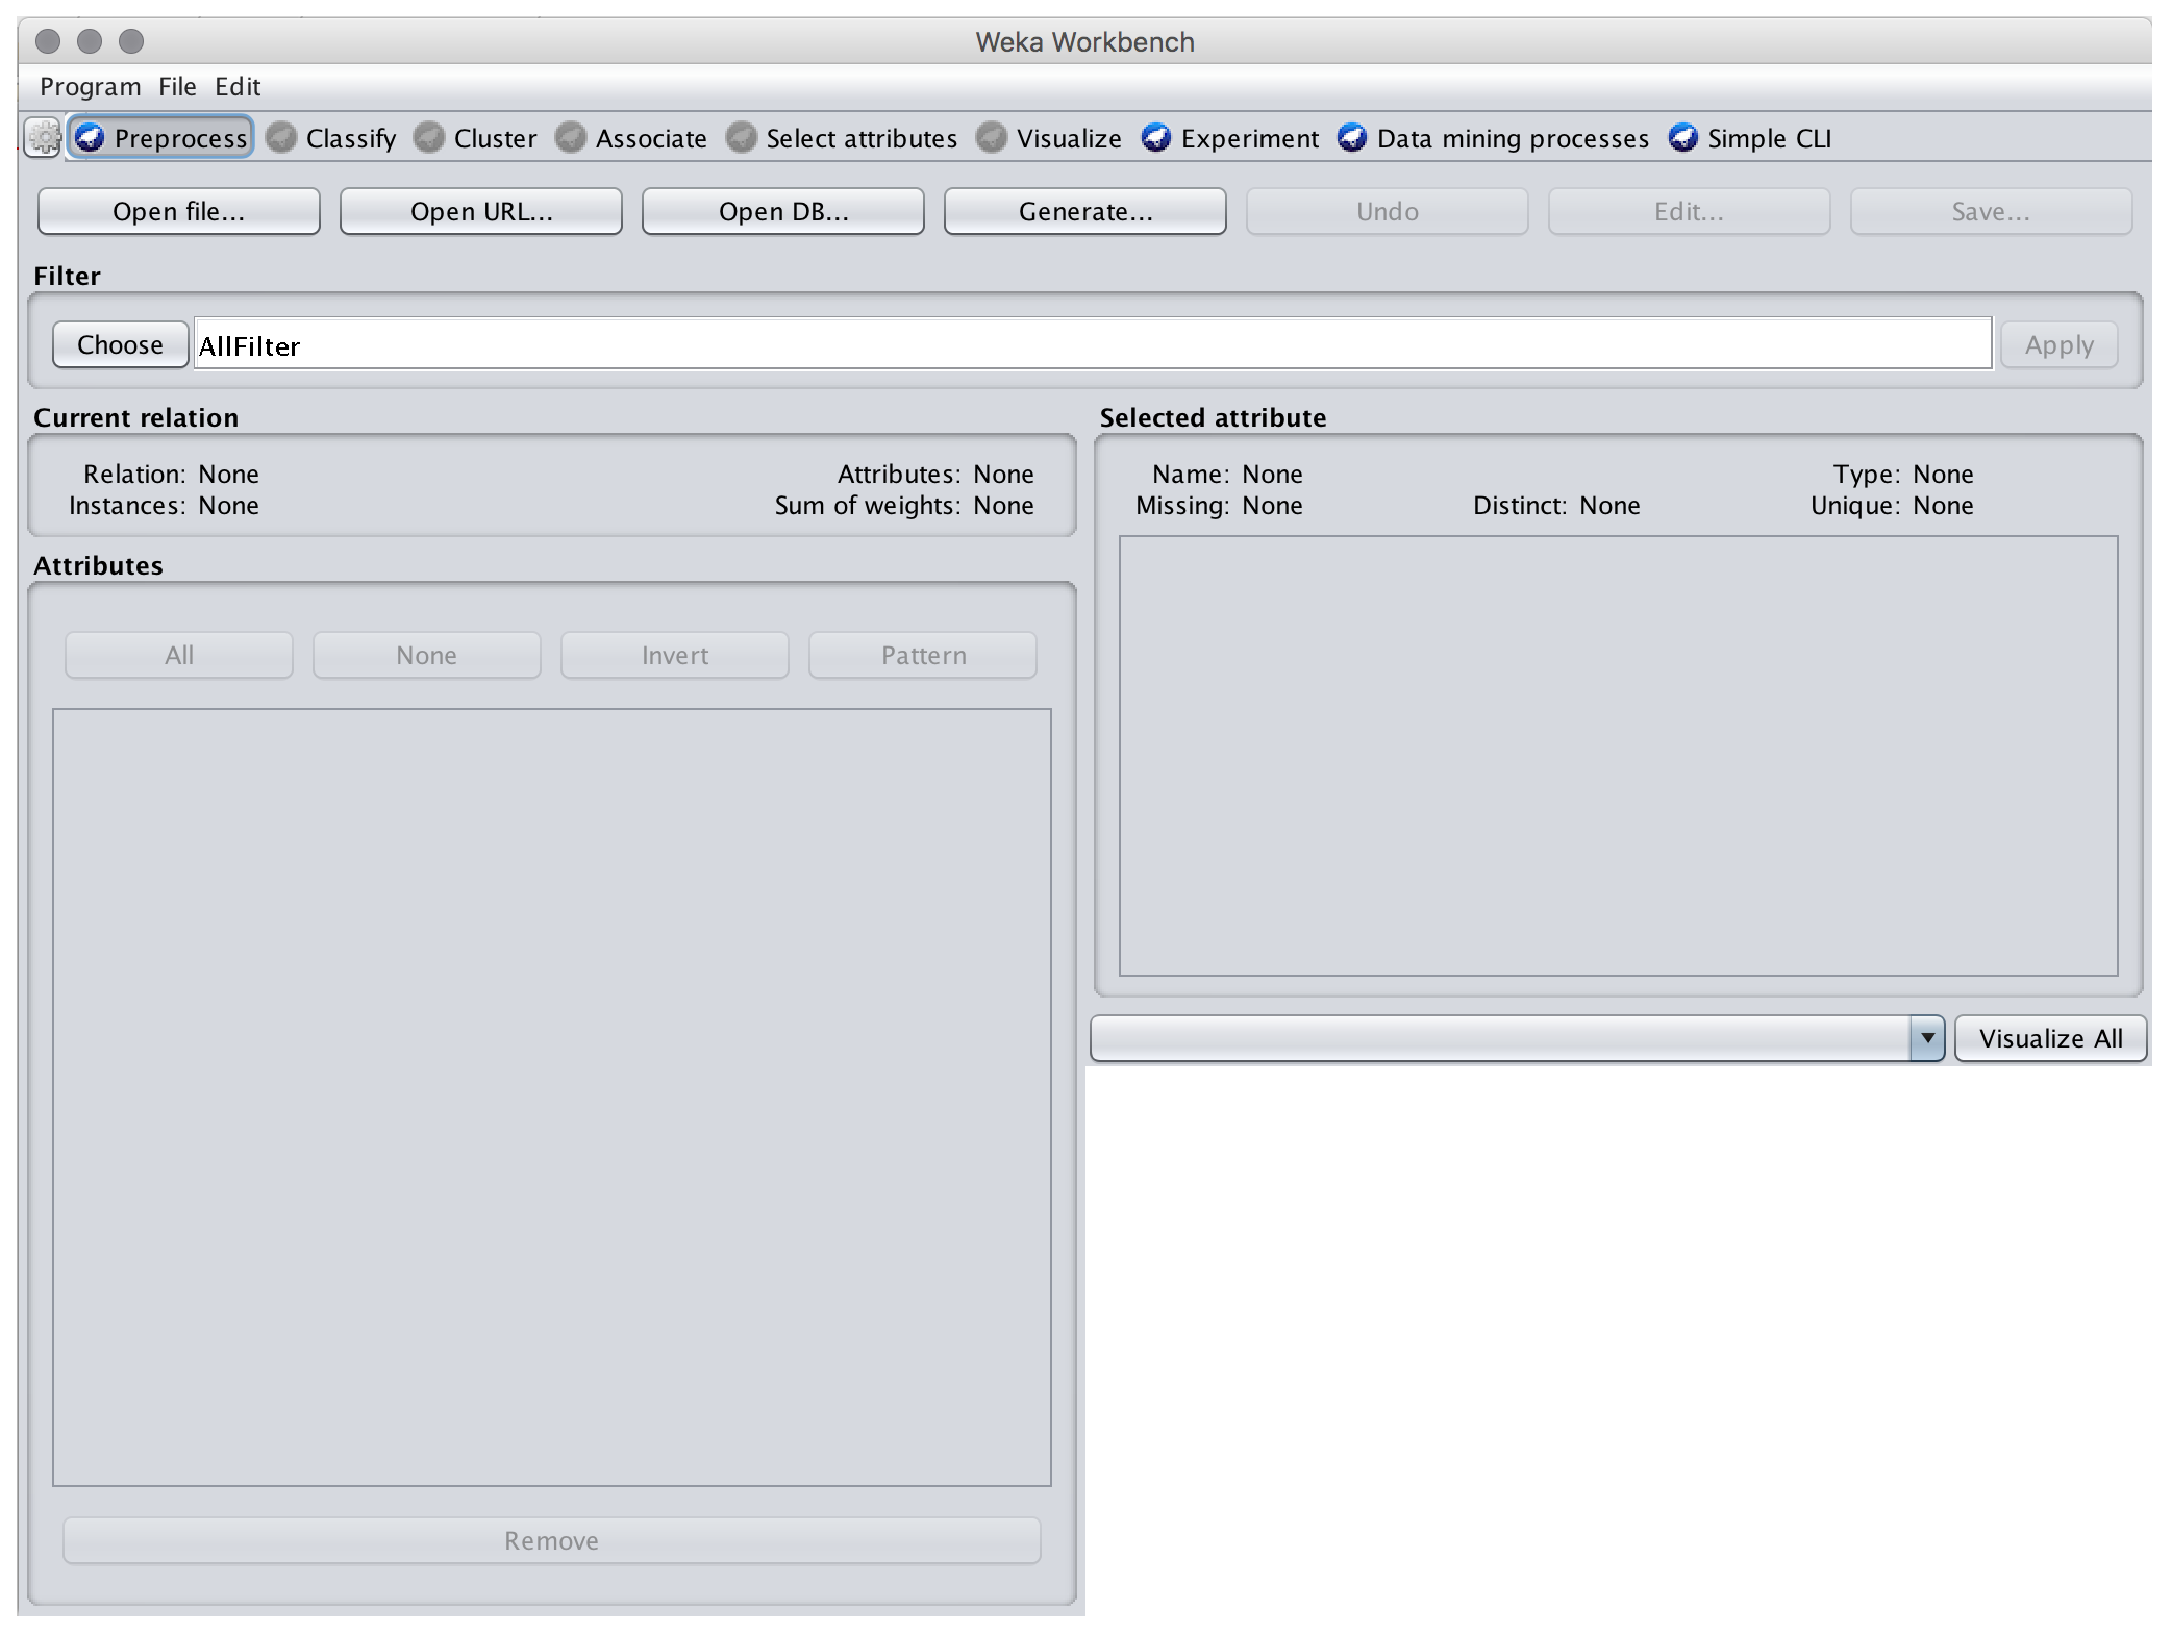
\includegraphics[width=10cm]{images/workbench/workbench.eps}
\end{center}

Because the Workbench is made up of other applications, there is not
much further to describe here with respect to its functionality. One
exception is that the Workbench exposes a number of general and
perspective-specific settings and preferences that the user can
modify. Settings are accessible by either the gear shaped icon in the
upper left-hand side of the GUI, or from the ``Program'' menu.

\begin{center}
  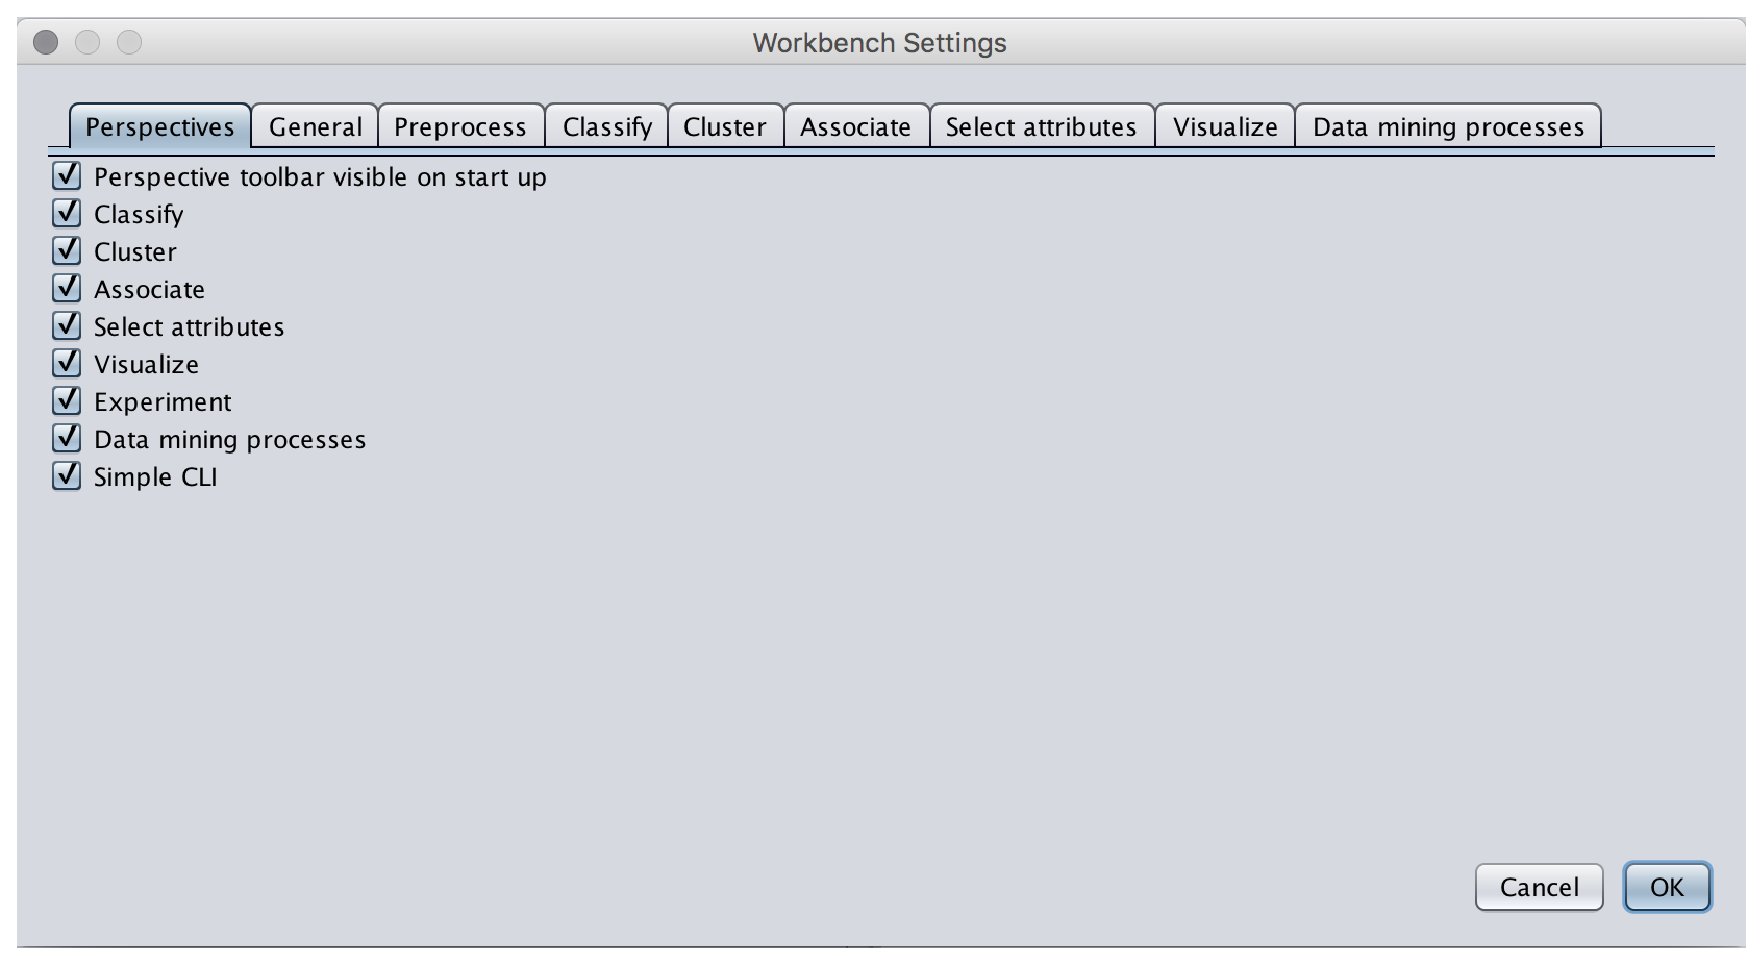
\includegraphics[width=10cm]{images/workbench/settings.eps}
\end{center}

From the settings the user can choose which perspectives should appear, and
modify general settings, such as the look-and-feel to use. Some settings
will come into affect immediately; while others, such as the look-and-feel,
will require that WEKA is restarted after making the change.

Beyond the \textit{Perspectives} and \textit{General} tabs in the settings
dialog each perspective will have its own tab for settings (as long as
a given perspective has user-configurable settings).

\begin{center}
  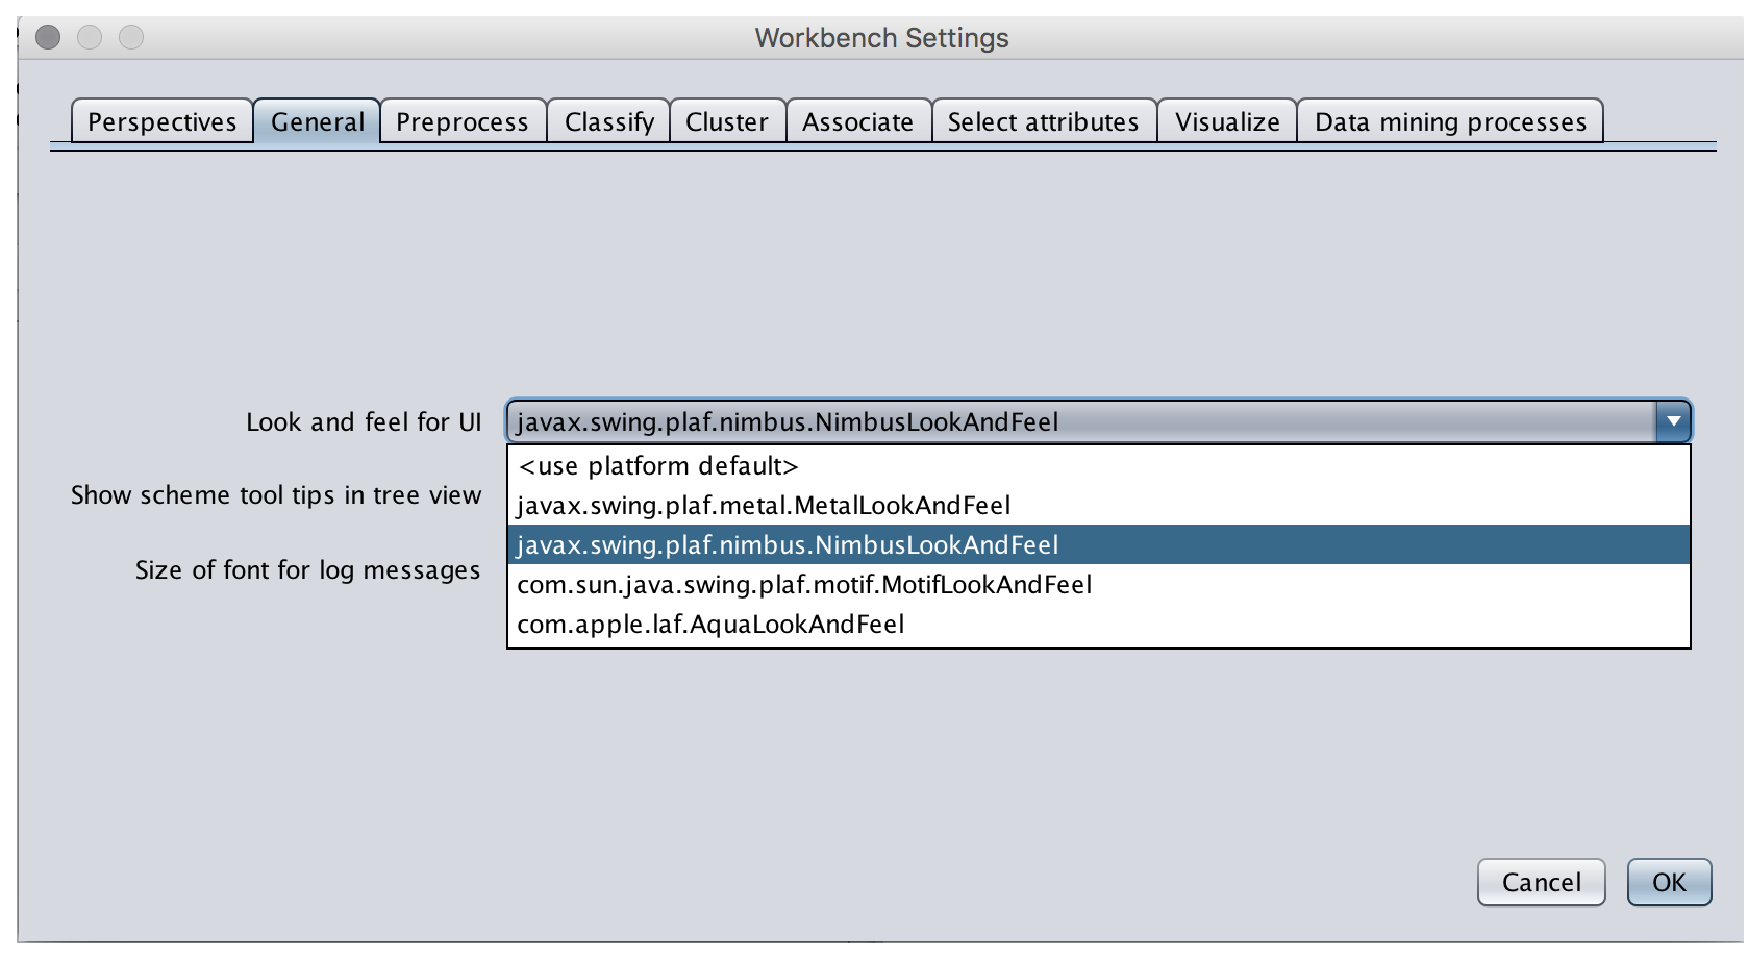
\includegraphics[width=10cm]{images/workbench/settings2.eps}
\end{center}

\begin{center}
  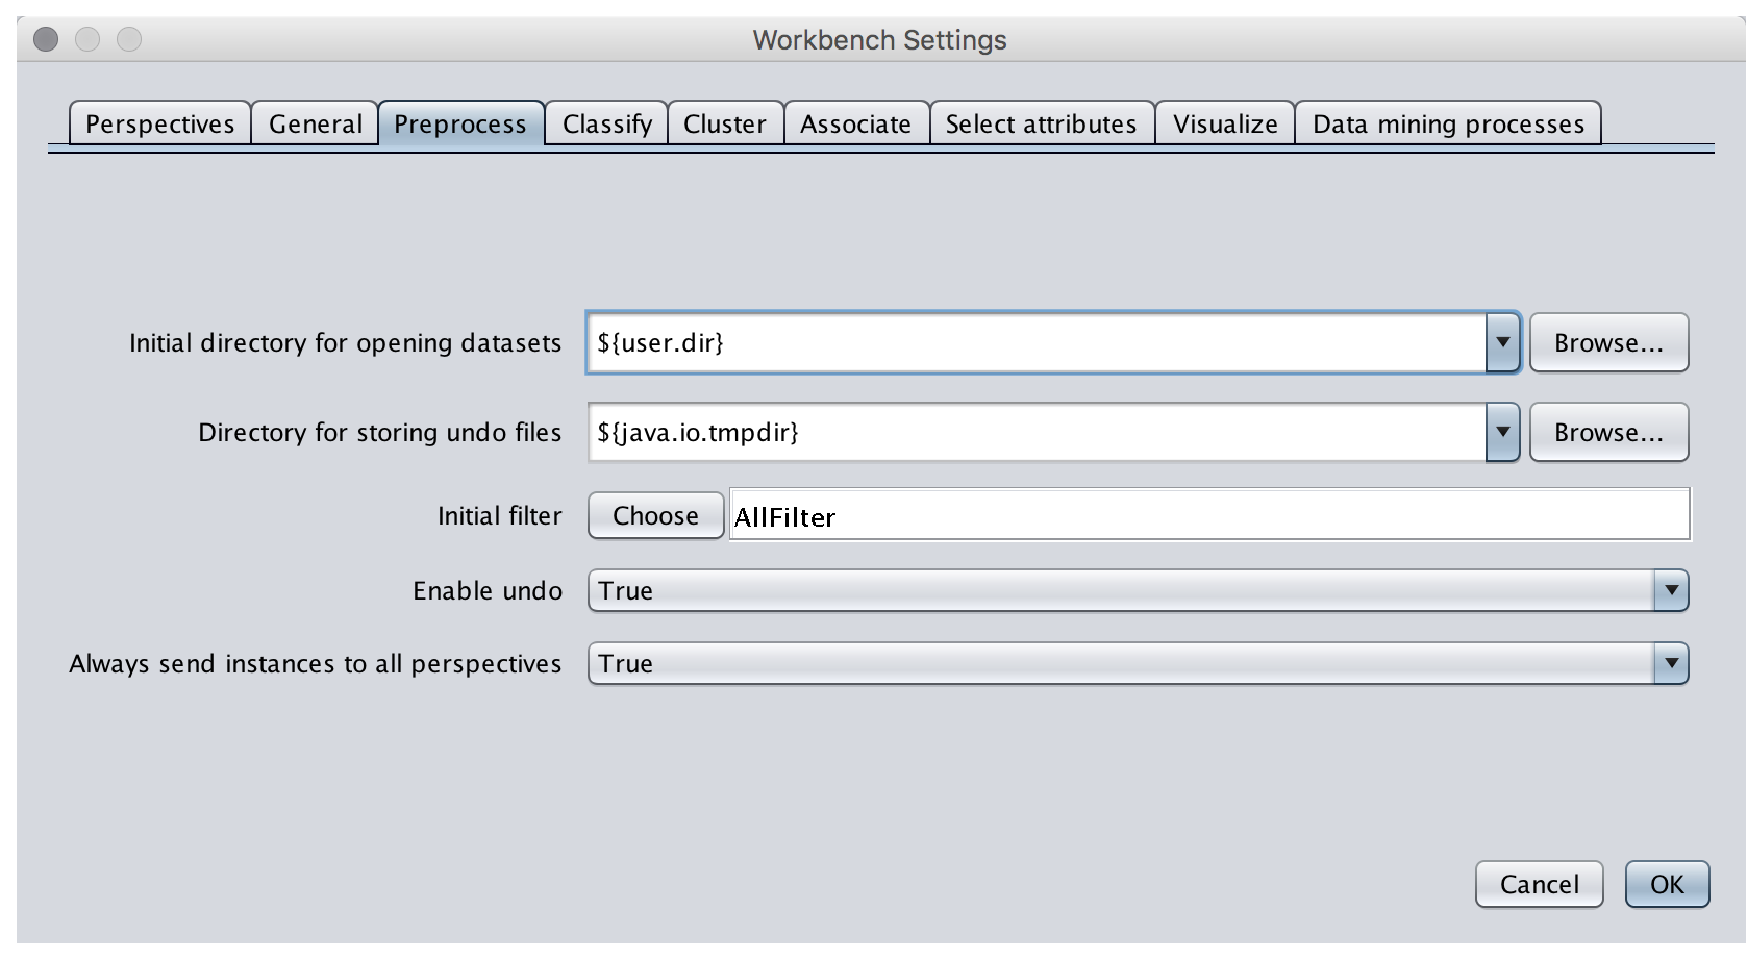
\includegraphics[width=10cm]{images/workbench/settings3.eps}
\end{center}


\chapter{ArffViewer}
\input{arffviewer}

\chapter{Bayesian Network Classifiers}
\input{bayesnet}

%%%%%%%%%%%%%%%%%%%%%%%%%%%%%%%%%%%
\part{Data}

\chapter{ARFF}
\input{arff}

\chapter{XRFF}
\label{xrff}
\input{xrff}

\chapter{Converters}
\input{converters}

\chapter{Stemmers}
\input{stemmers}

\chapter{Databases}
\input{databases}

\chapter{Windows databases}
\input{windows_databases}

%%%%%%%%%%%%%%%%%%%%%%%%%%%%%%%%%%%
\part{Appendix}
\chapter{Research}
\input{research}

\chapter{Using the API}
\input{using_api}

\chapter{Extending WEKA}
%
%   This program is free software: you can redistribute it and/or modify
%   it under the terms of the GNU General Public License as published by
%   the Free Software Foundation, either version 3 of the License, or
%   (at your option) any later version.
%
%   This program is distributed in the hope that it will be useful,
%   but WITHOUT ANY WARRANTY; without even the implied warranty of
%   MERCHANTABILITY or FITNESS FOR A PARTICULAR PURPOSE.  See the
%   GNU General Public License for more details.
%
%   You should have received a copy of the GNU General Public License
%   along with this program.  If not, see <http://www.gnu.org/licenses/>.
%

% Version: $Revision$

For most users, the existing WEKA framework will be sufficient to perform the
task at hand, offering a wide range of filters, classifiers, clusterers, etc.
Researchers, on the other hand, might want to add new algorithms and compare
them against existing ones. The framework with its existing algorithms is not
set in stone, but basically one big plugin framework. With WEKA's automatic
discovery of classes on the classpath, adding new classifiers, filters, etc. to
the existing framework is very easy.

Though algorithms like clusterers, associators, data generators and
attribute selection are not covered in this chapter, their implemention is very
similar to the one of implementing a classifier. You basically choose a
superclass to derive your new algorithm from and then implement additional
interfaces, if necessary. Just check out the other algorithms that are already
implemented.

The section covering the GenericObjectEditor (see chapter
\ref{genericobjecteditor}) shows you how to tell WEKA where to find your
class(es) and therefore making it/them available in the GUI
(Explorer/Experimenter) via the GenericObjectEditor.

%%%%%%%%%%%%%%%%%%%%%%%%%%%%
% Writing a new Classifier %
%%%%%%%%%%%%%%%%%%%%%%%%%%%%

\clearpage
\section{Writing a new Classifier}
\input{extending_classifier}

%%%%%%%%%%%%%%%%%%%%%%%%
% Writing a new Filter %
%%%%%%%%%%%%%%%%%%%%%%%%

\newpage
\section{Writing a new Filter}
\input{extending_filter}

%%%%%%%%%%%%%%%%%%%%%%%%%%%%
% Writing other algorithms %
%%%%%%%%%%%%%%%%%%%%%%%%%%%%

\newpage
\section{Writing other algorithms}
\input{extending_other_algorithms}

%%%%%%%%%%%%%%%%%%%%%%%%%%
% Extending the Explorer %
%%%%%%%%%%%%%%%%%%%%%%%%%%

\newpage
\section{Extending the Explorer}
\input{extending_explorer}

\newpage
\section{Extending the Knowledge Flow}
%
%   This program is free software: you can redistribute it and/or modify
%   it under the terms of the GNU General Public License as published by
%   the Free Software Foundation, either version 3 of the License, or
%   (at your option) any later version.
%
%   This program is distributed in the hope that it will be useful,
%   but WITHOUT ANY WARRANTY; without even the implied warranty of
%   MERCHANTABILITY or FITNESS FOR A PARTICULAR PURPOSE.  See the
%   GNU General Public License for more details.
%
%   You should have received a copy of the GNU General Public License
%   along with this program.  If not, see <http://www.gnu.org/licenses/>.
%

% Version: $Revision: 8032 $

The plugin architecture of the Knowledge Flow allows you to add new steps
and perspectives easily. Plugins for the Knowledge Flow are managed by the
/textit{PluginManager} class and can easily be deployed by creating a 
WEKA package (see Chapter 19) that includes a \textit{PluginManager.props}
file that lists the components to add.

The source code for all the examples described in the following
sections are available in the \textit{newKnowledgeFlowStepExamples}
package that can be installed via the package manager.

\subsection{Creating a simple batch processing Step}
Steps are the building blocks of Knowledge Flow processes. The new
Knowledge Flow implementation has a fresh API and a collection of
helper classes that makes creating a new Step fairly simple.

The need-to-know API elements for new Steps are:

\begin{itemize}
\item \texttt{weka.knowledgeflow.steps.Step} - the main interface for Step implementations
\item \texttt{weka.knowledgeflow.steps.BaseStepExtender} - a minimal subset of the
  \texttt{Step} interface's methods that a new Step would need to
  implement in order to function as a start point and/or processing
  step in the Knowledge Flow.
\item \texttt{weka.knowledgeflow.steps.BaseStep} - a handy base class
  for new Steps to extend. Provides functions for automatically setting up 
  the Step's name and ``about'' info, resolving environment variables
  and gaining access to the Step's \texttt{StepManager} class. This
  class implements \texttt{Step} and \texttt{BaseStepExtender}.
\item \texttt{weka.knowledgeflow.StepManager} - an implementation of
  \textit{StepManager} is provided to every Step by the Knowledge Flow
  environment. \texttt{StepManager} has lots of utility functions that
  allow a Step to find out information about things such as its
  incoming connections, outgoing connections, and execution
  environment. It also provides methods to handle the output of data
  and for informing the Knowledge Flow environment of the Step's
  status.
\item \texttt{weka.knowledgelfow.steps.KFStep} - a class annotation
  that Step implementations can use for specifying their name,
  category, tool tip and icon path.
\end{itemize}

Lets take a look at a simple Step that can accept batch datasets and
compute summary statistics for a user-specified attribute.

\subsection*{Implementation}

Our new \texttt{StatsCalculator} step extends \texttt{BaseStep}. As \texttt{BaseStep}
is abstract, the methods that we must implement are shown in the skeleton class below:

\begin{verbatim}
public class StatsCalculator extends BaseStep {

  @Override
  public void stepInit() throws WekaException {
    // TODO
  }

  @Override
  public List<String> getIncomingConnectionTypes() {
    // TODO
    return null;
  }

  @Override
  public List<String> getOutgoingConnectionTypes() {
    // TODO
    return null;
  }
}
\end{verbatim}

The \textit{stepInit()} function is called on all steps before the
knowledge flow starts executing a flow. It allows a step to reset its
state and check the validity of any user-specified configuration. At
this point the Step is guaranteed to have access to a
\texttt{StepManager}.

The \textit{getIncomingConnectionTypes()} method allows a Step to
specify which incoming connection types it can accept. This should
take into account the current configuration of the step and any
existing connections in (or out) of the step (e.g. a step might only
allow one incoming \textit{trainingSet} connection, so if one is
already present then the list of connection types returned by this
method should not include \textit{trainingSet}).

Similarly, the \textit{getOutgoingConnectionTypes()} method allows the
Step to specify which outgoing connection types can be made from
it. Again, this should take into account the current state of the step
and (possibly) the incoming connections.

Lets take a look at implementing these methods in
\verb=StatsCalculator=.:

\begin{verbatim}
public class StatsCalculator extends BaseStep {

  protected String m_attName = "petallength";

  @Override
  public void stepInit() throws WekaException {
    if (m_attName == null || m_attName.length() == 0) {
      throw new WekaException("You must specify an attribute to compute "
        + "stats for!");
    }
  }

  @Override
  public List<String> getIncomingConnectionTypes() {
    return Arrays.asList(StepManager.CON_DATASET, StepManager.CON_TRAININGSET,
      StepManager.CON_TESTSET);
  }

  @Override
  public List<String> getOutgoingConnectionTypes() {
    List<String> outgoing = new ArrayList<String>();
    if (getStepManager().numIncomingConnections() > 0) {
      outgoing.add(StepManager.CON_TEXT);
    }
    if (getStepManager().numIncomingConnectionsOfType(
      StepManager.CON_DATASET) > 0) {
      outgoing.add(StepManager.CON_DATASET);
    }
    if (getStepManager().numIncomingConnectionsOfType(
      StepManager.CON_TRAININGSET) > 0) {
      outgoing.add(StepManager.CON_TRAININGSET);
    }
    if (getStepManager().numIncomingConnectionsOfType(
      StepManager.CON_TESTSET) > 0) {
      outgoing.add(StepManager.CON_TESTSET);
    }
    return outgoing;
  }
}
\end{verbatim}

The code specifies that the step can accept any number of incoming
\texttt{dataset}, \texttt{trainingSet} or \texttt{testSet}
connections. There are a whole lot of constants defined in
\texttt{StepManager} for connection types and auxilliary data. The
\textit{getOutgoingConnectionTypes()} method specifies that the step
will only produce a \texttt{text} connection/output if it has at least
one incoming connection. The \texttt{text} output will contain our
computed attribute summary statistics. Furthermore, the step also
passes through any instances that it receives, so it will only produce
a particular dataset type (\texttt{dataSet}, \texttt{trainingSet} or
\texttt{testSet}) if it has a corresponding inpcoming connection of
that type.

At this point there is some important functionality missing - namely a
method to do some actual processing when data is received by the
step. In fact, there are two methods related to this in
\texttt{BaseStep} that have no-opp implementations. One or both should
be overridden by a \verb=Step= implementation in order to do some
processing. the \textit{start()} method should be overriden if the
step can act as a starting point in a flow (i.e. a step that,
typically, loads, sources or generates data of some sort). Any step
that doesn't have any incoming connections is considered as a
potential start point by the Knowledge Flow environment and has its
\textit{start()} method invoked. The \textit{processIncoming()} method
should be overridden by steps that can accept incoming connections
(and the data that they typically carry).

Lets add a \textit{processIncoming()} method to the \verb=StatsCalculator=.

\begin{verbatim}
  public void setAttName(String attName) { m_attName = attName; }

  public String getAttName() { return m_attName; }

  @Override
  public void processIncoming(Data data) throws WekaException {
    getStepManager().processing();
    Instances insts = data.getPrimaryPayload();
    Attribute att = insts.attribute(getAttName());
    if (att == null) {
      throw new WekaException("Incoming data does not " + "contain attribute '"
        + getAttName() + "'");
    }
    AttributeStats stats = insts.attributeStats(att.index());
    Data textOut = new Data(StepManager.CON_TEXT, stats.toString());
    textOut.setPayloadElement(StepManager.CON_AUX_DATA_TEXT_TITLE,
      "Stats for: " + getAttName());
    getStepManager().outputData(textOut); // output the textual stats
    getStepManager().outputData(data); // pass the original dataset on
    getStepManager().finished();
  }
\end{verbatim}

In the code above, we've added accessor and mutator methods for our
single user-supplied parameter - i.e. the name of the attribute to
compute stats for. Then we've overridden the no-opp implementation of
the \textit{processIncoming()} method from \verb=BaseStep=. This
method is passed a \verb=Data= object, which is the data structure
used by the Knowledge Flow environment for transferring all types of
data between steps. The code first tells the Knowledge Flow
environment that it is actively processing by calling the
\textit{processing()} method on the step's \verb=StepManager=. It then
retrieves the \verb=Instances= dataset via the
\textit{getPrimaryPayload()} method of the \verb=Data= object. The
stats are then computed and a new \verb=Data= object is created to
hold the results. In this case the results are textual, so the data's
associated connection type is \verb=StepManager.CON_TEXT=. The two
argument constructor for \verb=Data= takes the connection type and the
associated primary payload data (i.e. the textual stats in this
case). Additional data can be attached to a \verb=Data= object by
storing it in a ``payload'' map. In this case we have a textual title
for our stats result that includes the name of the attribute. Finally,
the new data object, and the original dataset, is output by calling
the \textit{outputData()} method on the \verb=StepManager=, and the
environment is informed that our step has finished processing.

The last thing we can add to this step is the \verb=KFStep= class
annotation. This provides some information about the step, including
where it should appear in the folders of the design palette in the
GUI Knowledge Flow.

\begin{verbatim}
@KFStep(name = "StatsCalculator", category = "Examples",
  toolTipText = "Compute summary stats for an attribute",
  iconPath = KFGUIConsts.BASE_ICON_PATH + "DiamondPlain.gif")
public class StatsCalculator extends BaseStep {

...
\end{verbatim}


\begin{center}
  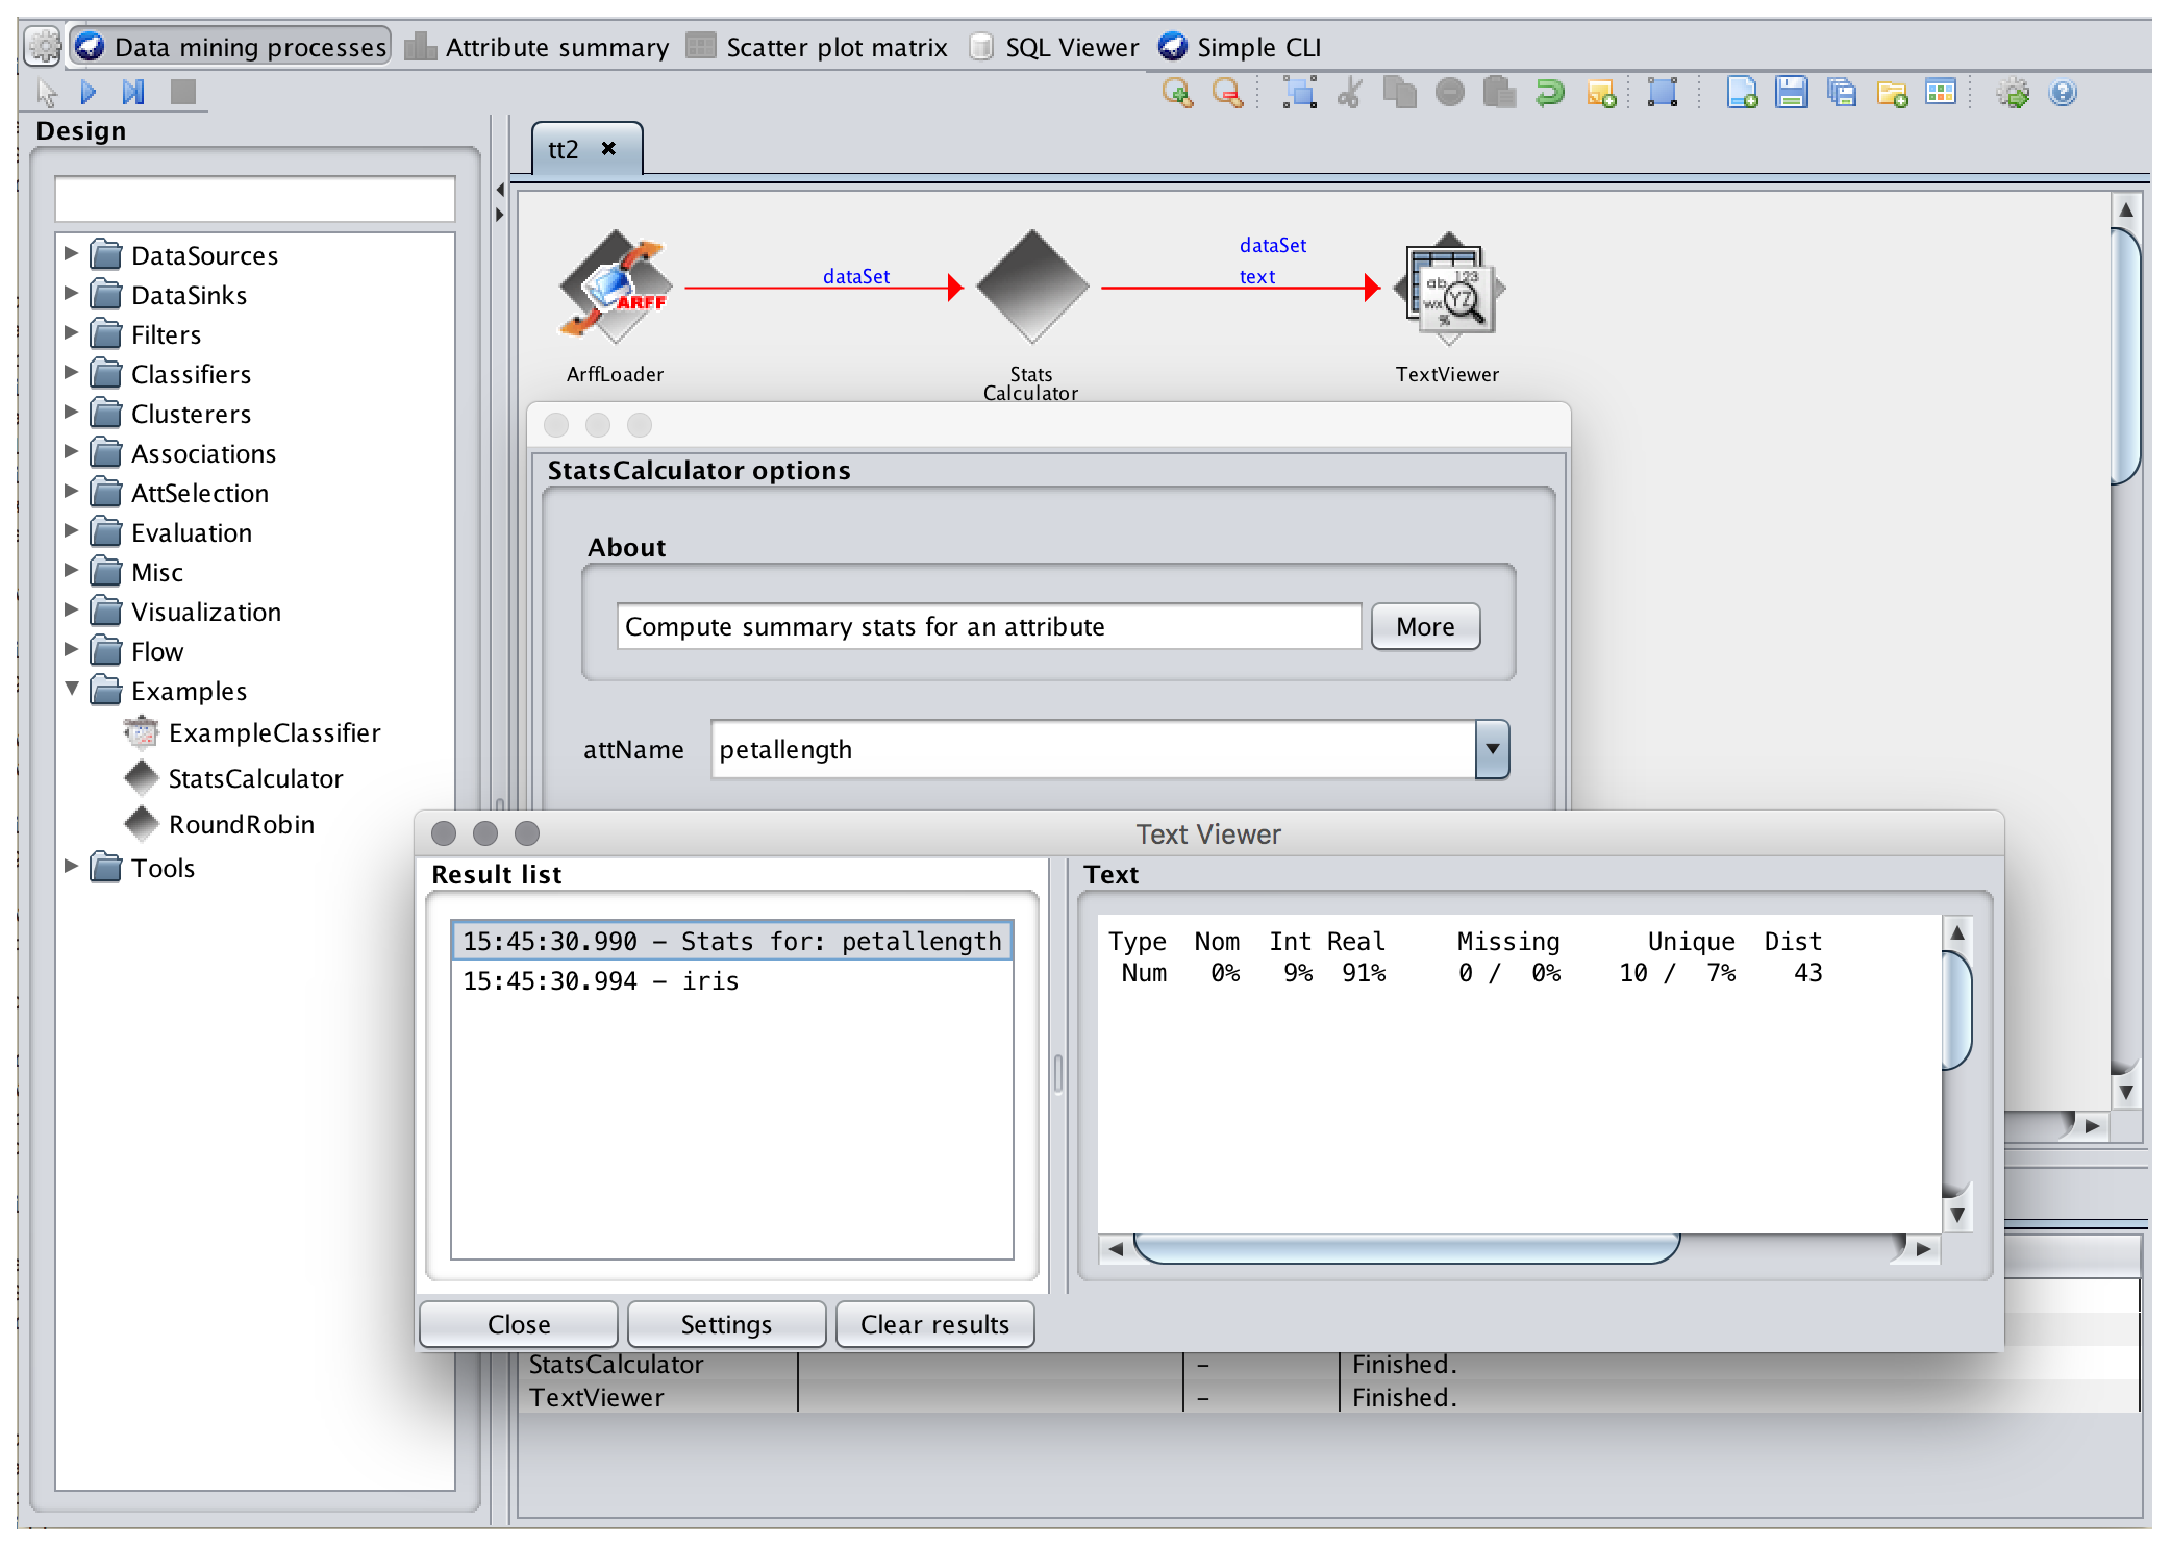
\includegraphics[width=12cm]{images/knowledgeflow/statsCalc.eps}
\end{center}

The screenshot above shows the step, the results after execution on
the iris data and the GUI configuration dialog for the step. A simple,
GUI configuration dialog is provided dynamically by the Knowledge Flow
environment, but you have the option of overriding this to a greater
or lesser extent in order to provide a customized configuration
dialog.

\subsection{Creating a simple streaming Step}
\verb=StepManager= defines a number of constant strings that identify
various types of connections and data. Most data/connections in the
Knowledge Flow are batch ones - e.g. \textit{dataSet},
\textit{trainingSet}, \textit{testSet} and \textit{batchClassifier}
(to name a few). When the Knowledge Flow's execution environment
invokes \textit{processIncoming()} on a target step, it does so in a
separate thread for batch connections. Thus, each step automatically
does its processing within a separate thread. There are several types
of incremental connections/data defined in \verb=StepManager= as well:
\textit{instance}, \textit{incrementalClassifier} and \textit{chart}
are all examples. Furthermore, for your own purposes it is possible to
create your own connection/data types (as they are just defined with a
string identifier) and mark them as ``incremental''. This can be done
by setting payload flag
(\verb=StepManager.CON_AUX_DATA_IS_INCREMENTAL= to \verb=true=) when
configuring a \verb=Data= object. Incremental connections/data do not
get executed in a new thread because it is assumed that processing
individual pieces of incremental data does not require much effort,
and the overhead in creating/invoking processing in a new thread could
outweigh this.

Now lets take a look at a \verb=Step= that does some simple processing
in a streaming fashion. Our new step, \verb=RoundRobin=, simply
accepts a single streaming ``instance'' connection as input and
distributes individual instances in a round-robin fashion to the
connected steps immediately downstream from it.

\subsection*{Implementation}

\begin{verbatim}
@KFStep(name = "RoundRobin", category = "Examples",
  toolTipText = "Round robin instances to outputs",
  iconPath = KFGUIConsts.BASE_ICON_PATH + "DiamondPlain.gif")
public class RoundRobin extends BaseStep {
  protected int m_counter;
  protected int m_numConnected;

  @Override
  public void stepInit() throws WekaException {
    m_counter = 0;
    m_numConnected = getStepManager().numOutgoingConnections();
  }

  @Override
  public List<String> getIncomingConnectionTypes() {
    List<String> result = new ArrayList<String>();
    if (getStepManager().numIncomingConnections() == 0) {
      result.add(StepManager.CON_INSTANCE);
    }
    return result;
  }
  @Override
  public List<String> getOutgoingConnectionTypes() {
    List<String> result = new ArrayList<String>();
    if (getStepManager().numIncomingConnections() == 1) {
      result.add(StepManager.CON_INSTANCE);
    }
    return result;
  }

  @Override
  public void processIncoming(Data data) throws WekaException {
    if (isStopRequested()) {
      getStepManager().interrupted();
      return;
    }
    if (getStepManager().numOutgoingConnections() > 0) {
      getStepManager().throughputUpdateStart();
      if (!getStepManager().isStreamFinished(data)) {
        List<StepManager> outgoing =
          getStepManager().getOutgoingConnectedStepsOfConnectionType(
            StepManager.CON_INSTANCE);
        int target = m_counter++ % m_numConnected;
        String targetStepName = outgoing.get(target).getName();
        getStepManager().outputData(StepManager.CON_INSTANCE, targetStepName,
          data);
        getStepManager().throughputUpdateEnd();
      } else {
        // step manager notifies all downstream steps of stream end
        getStepManager().throughputFinished(data);
      }
    }
  }
}
\end{verbatim}
\newpage

This example step demonstrates a several different things over the one
in the previous section. Firstly the
\textit{getIncomingConnectionTypes()} and
\textit{getOutgoingConnectionTypes()} methods demonstrate some
constraints based on the current state of incoming and outgoing
connections. In the former method a constraint of a single incoming
\verb=instance= connection is enforced; in the later method any number
of outgoing \verb=instance= connections are allowed as long as there
is an incoming connection present. It also demonstrates checking to
see whether a request has been made to stop processing in the
\textit{processIncoming()} method. We ommitted this from the previous
example for brevity, but all steps should check periodically to see if
a stop has been requested. If so, then they should indicate to the
environment as soon as possible that they have been interrupted by
calling \textit{StepManager.interrupted()}. This method will ensure
that an interruped message appears in the status area of the GUI
Knowledge Flow.

The code also demonstrates several features of incremental processing
in the \textit{processIncoming()} method. To get throughput statistics
displayed in the status area of the GUI Knowledge Flow interface the
methods \textit{StepManager.throughputUpdateStart()} and
\textit{StepManager.throughputUpdateEnd()} are used to indicate the
start and end of processing for the incoming \verb=Data= object
respectively. A utility method \textit{StepManager.isStreamFinished()}
can be called to see if the end of the stream has been reached. This
method takes the current \verb=Data= object (as a flag is set in the
payload map of the \verb=Data= object to indicate the end of the
stream). By convention, the primary payload of a \verb=Data= object
that is marked as end-of-stream is empty/null. However, auxilliary
data could be present, depending on what processing has been done
(e.g. a final classifier object if training a classifier
incrementally). If the end of stream has been reached, then a step
should call \textit{StepManager.throughputFinished()} with a final
\verb=Data= object as an argument - this tells the environment that
processing is finished for the step and ensures that downstream steps
are informed of the end-of-stream along with any final auxilliary data
in the final \verb=Data= object.

In the previous example, we had simply output data to all downstream
steps with the appropriate connection type by calling
\textit{StepManager.outputData()} with a single \verb=Data= object as
an argument. The environment routes this data to appropriate connected
steps because the \verb=Data= object is constructed with a connection
type that it is associated with. In our round robin example, we
further constrain the destination of the data by calling a version of
\textit{StepManager.outputData()} that takes a step name as an additional
argument.

\subsection{Features of StepManager}

Aside from methods to query the state of incoming and outgoing connections
from a step, and support for outputing data, the \verb=StepManager= also
has a number of other useful facilities. It provides methods for writing
to the status and log in the KnowledgeFlow. Messages can be logged at
various logging levels, where the user can configure up to which level
they are interested in seeing in the log. The following status and logging
methods can be used by steps during execution:

\begin{tight_itemize}
  \item \verb=statusMessage()= - write to the status area
    \item \verb=logLow()=
    \item \verb=logBasic()=
    \item \verb=logDetailed()=
    \item \verb=logDebug()=
    \item \verb=logWarning()= - always gets to the log, regardless of user-specified logging level
    \item \verb=logError()= - always gets to the log; can supply an optional \verb=Throwable= cause
\end{tight_itemize}

\verb=StepManager= also provides access to the
\verb=ExecutionEnvornment=. The \verb=ExecutionEnvironment= can be
used to find out whether the system is running headless, get the
values of environment variables and to launch separate processing
``tasks'' on the executor service. In most cases, the processing done
by a step will not require launching additional tasks/threads as
\textit{processIncoming()} is called in a separate thread (when batch
processing) by the Knowledge Flow environment. In some cases, it might
be beneficial to make use of additional threads. The
\textit{BoundaryPlotter} step is an example that makes use of this
facility - it computes each row of a plotted graphic using a separate
task/thread. Steps wanting to use the executor service directly can
call \textit{StepManager.getExecutionEnvironment().submitTask()} and
supply a concrete sublcass of \verb=StepTask= to do the
processing. The step can work with either the
\verb=Future<ExectutionResult>= returned by \textit{submitTask()} or,
alternatively, supply a \verb=StepTaskCallback= when constructing a
\verb=StepTask= for asynchronous notification.

\subsection{PairedDataHelper}

A common processing pattern in machine learning is to deal with paired
datasets - i.e. typically train/test pairs. In the multi-threaded
environment of the Knowledge Flow, where usually each \verb=Data=
object is passed to a target step in a separate thread of execution,
it is likely that training and test sets may arrive at the target step
out of order. Furthermore, in the case of multiple pairs
(e.g. cross-validation folds) they might not arrive in the order that
the folds are created. Handling this scenario within a step can be
tedious, so a helper class is available for use by step
implementations needing to deal with paired datasets -
\verb=PairedDataHelper=.

The \verb=PairedDataHelper= has the concept of a primary and secondary
connection/data type, where the secondary connection/data for a given
set number typically needs to be processed using a result generated
from the corresponding primary connection/data. This class takes care
of ensuring that the secondary connection/data is only processed once
the primary has completed. Users of this helper need to provide an
implementation of the \verb=PairedProcessor= inner interface, where
the \textit{processPrimary()} method will be called to process the
primary data/connection (and return a result), and
\textit{processSecondary()} called to deal with the secondary
connection/data. The result of execution on a particular primary data
set number can be retrieved by calling the
\textit{getIndexedPrimaryResult()} method, passing in the set number
of the primary result to retrieve.

The \verb=PairedDataHelper= class also provides an arbitrary storage
mechanism for additional results beyond the primary type of result. It
also takes care of invoking \textit{processing()} and
\textit{finished()} on the client step's \verb=StepManager=.

Below is a code skeleton (taken from the javadoc for
\verb=PairedDataHelper=) that shows the basic usage of this helper
class.

\begin{verbatim}
public class MyFunkyStep extends BaseStep
  implements PairedDataHelper.PairedProcessor<MyFunkyMainResult> {
   ...
   protected PairedDataHelper<MyFunkyMainResult> m_helper;
   ...
   public void stepInit() {
     m_helper = new PairedDataHelper<MyFunkyMainResult>(this, this,
     StepManager.[CON_WHATEVER_YOUR_PRIMARY_CONNECTION_IS],
     StepManager.[CON_WHATEVER_YOUR_SECONDARY_CONNECTION_IS]);

      ...
    }

    public void processIncoming(Data data) throws WekaException {
      // delegate to our helper to handle primary/secondary synchronization
      // issues
      m_helper.process(data);
    }

    public MyFunkyMainResult processPrimary(Integer setNum, Integer maxSetNun,
      Data data, PairedDataHelper<MyFunkyMainResult> helper) throws WekaException {
      SomeDataTypeToProcess someData = data.getPrimaryPayload();
 
      MyFunkyMainResult processor = new MyFunkyMainResult();
      // do some processing using MyFunkyMainResult and SomeDataToProcess
      ...
      // output some data to downstream steps if necessary
      ...
   
      return processor;
    }
   
    public void processSecondary(Integer setNum, Integer maxSetNum, Data data,
      PairedDataHelper<MyFunkyMainResult> helper) throws WekaException {
      SomeDataTypeToProcess someData = data.getPrimaryPayload();
   
      // get the MyFunkyMainResult for this set number
      MyFunkyMainResult result = helper.getIndexedPrimaryResult(setNum);
   
      // do some stuff with the result and the secondary data
           ...
      // output some data to downstream steps if necessary
    }
}

\end{verbatim}

The \textit{newKnowledgeFlowStepExamples} package includes an example
called \verb=ExampleClassifier= that demonstrates the use of
\verb=PairedDataHelper= to train and evaluate a classifier on
train/test splits.



\chapter{Weka Packages}
\input{weka_packages}

\chapter{Technical documentation}
\input{technical_documentation}

\chapter{Other resources}
\input{other_resources}

%%%%%%%%%%%%%%%%%%%%%%%%%%%%%%%%%%%
\input{bibliography}

\end{document}
